%=============================================================================
%  EfficientNet-GCN : Explainable Osteoporosis Severity Classification
%  Revised manuscript -- journal format
%
%  -------------------------------------------------------------------------
%  OUTSTANDING ITEMS BEFORE SUBMISSION
%  Every unresolved value is marked in the text with \PEND, which typesets a
%  red [TBD].  Search for "\PEND" to find them all.  They fall into 3 groups:
%
%  (A) REQUIRES RETRAINING -- blocking for a Q1 submission
%      A1. Ablation variants (i)-(vi)          -> Table \ref{tab:ablation}
%      A2. Parameter-matched conv control       -> Table \ref{tab:ablation}, row (vii)
%      A3. Baselines on the identical split     -> Table \ref{tab:baselines}
%      A4. Cross-validation / multi-seed runs   -> Sec. \ref{sec:statistics}
%      A5. Ensemble-weight sensitivity sweep    -> Sec. \ref{sec:auxensemble}
%
%  (B) COMPUTABLE FROM ARTIFACTS YOU ALREADY HAVE -- no retraining needed
%      B1. Quadratic weighted kappa + grade MAE -> from the saved confusion matrix
%      B2. Top-2 accuracy                       -> from saved probability outputs
%      B3. Per-class AUC                        -> from saved probability outputs
%      B4. ECE / reliability diagram            -> from saved probability outputs
%      B5. Bone-intensity means and SDs         -> Sec. \ref{sec:preprocessing}
%      B6. GFLOPs, CPU latency, peak memory     -> Table \ref{tab:efficiency}
%
%  (C) EDITORIAL
%      C1. Author 2 and author 3 shared one e-mail in the source file.
%          Author 3's address below is marked FIXME -- correct it.
%      C2. Decide on code release; update the Data and Code Availability
%          section accordingly.
%      C3. Confirm the PyTorch Geometric version and system RAM.
%
%  Wilson confidence intervals reported in Sec. \ref{sec:testperf} were derived
%  analytically from the already-reported counts; they require no new runs.
%=============================================================================

\documentclass[journal]{IEEEtran}
\IEEEoverridecommandlockouts

\usepackage{cite}
\usepackage{amsmath,amssymb,amsfonts}
\usepackage{graphicx}
\usepackage{textcomp}
\usepackage{xcolor}
\usepackage{float}
\usepackage{booktabs}
\usepackage{array}
\usepackage{url}

% Placeholder marker for values that are not yet available.
% Remove this definition once every \PEND has been replaced.
\newcommand{\PEND}{\textcolor{red}{\textbf{[TBD]}}}

\begin{document}

\title{EfficientNet-GCN: A Hybrid Convolutional--Graph Framework for
Explainable Multi-Class Osteoporosis Severity Classification from
Knee Radiographs}

\author{Tasnim~Sultana~Sintheia,
        Musfique~Rahman~Muin,
        Pranta~Das~Gupta,
        and~Md.~Iftekharul~Mobin%
\thanks{T. S. Sintheia, M. R. Muin, and P. D. Gupta are with the Department of
Computer Science and Engineering, American International University-Bangladesh
(AIUB), Dhaka, Bangladesh (e-mail: 26-93981-1@student.aiub.edu;
26-94167-2@student.aiub.edu;
% FIXME (C1): the source manuscript gave authors 2 and 3 the same address.
% Replace the line below with author 3's correct student e-mail.
26-94167-2@student.aiub.edu).}%
\thanks{M. I. Mobin is with the Department of Computer Science and Engineering,
American International University-Bangladesh (AIUB), Dhaka, Bangladesh
(e-mail: iftekhar.mobin@aiub.edu).}}

\maketitle

\begin{abstract}
Osteoporosis often remains undetected until a fragility fracture occurs, and
limited access to dual-energy X-ray absorptiometry (DXA) leaves routine knee
radiographs an underused screening opportunity in resource-constrained
settings. Existing deep learning approaches to this task reason over the
radiograph as a Euclidean grid, representing relationships between
anatomically adjacent bone regions only implicitly through the convolutional
receptive field, and typically expose a single coarse saliency map as their
only account of a decision. This paper presents EfficientNet-GCN, a hybrid
convolutional--graph framework for explainable three-class osteoporosis
severity classification from knee radiographs. It comprises a
\emph{Patch-Graph Construction Module} that channel-reduces EfficientNetB0's
spatial feature map and reformulates it as an eight-connected, 100-node patch
graph; a \emph{Residual Dual-Pooling Graph Reasoning Branch} that propagates
relational context across three graph-convolutional layers and reads it out
through concatenated mean--max pooling; and an \emph{Auxiliary Convolutional
Branch} fused with the graph branch by a weighted probability head. The
1,947-image corpus is partitioned before any augmentation is applied, and only
the training partition is rebalanced to 3,000 images, so the validation and
test partitions retain their natural class distribution throughout evaluation.
On the 293-image held-out test set the model attains 82.94\% accuracy (95\%
Wilson confidence interval 78.2--86.8\%), a macro F1-score of 0.8161, and a
macro one-vs-rest AUC of 0.9429, with 5.03M parameters. A three-tier
explainability suite, Grad-CAM over the convolutional backbone, GNNExplainer
over the patch graph, and LIME over super-pixels, localizes predictions to
cortical and trabecular bone regions rather than background or soft tissue.
The contribution of this work is a leakage-controlled evaluation protocol, an
explicit relational representation over patch-level features, and the joint
reporting of three complementary explanation views alongside a full parameter
budget.
\end{abstract}

\begin{IEEEkeywords}
Osteoporosis, bone mineral density, knee radiograph, EfficientNet, graph
convolutional network, explainable artificial intelligence, Grad-CAM,
opportunistic screening, medical image classification.
\end{IEEEkeywords}

\section{Introduction} \label{Introduction}
\IEEEPARstart{O}{steoporosis} is a progressive systemic skeletal disorder
characterized by reduced bone mineral density (BMD) and deterioration of bone
microarchitecture, resulting in fragility fractures \cite{lorentzon2022osteoporosis}.
It is often described as a silent disease because it produces no symptoms
until a fracture occurs, at which point it causes ongoing pain, loss of
independence, and increased mortality, particularly among the elderly
\cite{salari2021global}. As the global population ages, the incidence of
osteoporosis is expected to rise, placing a significant socio-economic burden
on healthcare systems worldwide. Dual-energy X-ray absorptiometry (DXA) is the
diagnostic gold standard, but the cost of the equipment, its concentration in
tertiary centres, and the referral pathway it requires together prevent its use
as a population-level screening tool \cite{hui2025deep}. Timely osteoporosis
screening therefore remains scarce, especially in resource-poor and rural
healthcare settings \cite{auriat2026evaluating}.

Conventional knee radiography, by contrast, is inexpensive, widely available,
and routinely acquired during musculoskeletal assessment for osteoarthritis and
trauma \cite{wani2023osteoporosis}. Radiographs already acquired for these
indications therefore present an opportunity for opportunistic osteoporosis
screening without additional acquisitions or additional radiation exposure
\cite{hui2025deep}. Manual assessment of trabecular pattern and cortical
appearance on knee radiographs is, however, difficult and subject to high
inter-observer variability, which limits its usefulness for early diagnosis
\cite{wani2023osteoporosis}. Recent advances in deep learning, and Convolutional
Neural Networks (CNNs) in particular, have shown considerable promise for
automatically learning the complex imaging patterns and sub-visual bone texture
features associated with bone degeneration
\cite{sukegawa2022identification,wani2023osteoporosis}.

Although CNN architectures such as ResNet and VGG have demonstrated strong
performance on this task \cite{wani2023osteoporosis}, several limitations
remain. Current approaches extract local spatial features within fixed
receptive fields and do not explicitly model relationships between
anatomically related regions of the knee across scales \cite{mienye2025graph}.
Most existing methods are additionally black boxes, offering little
interpretability and thereby reducing clinician confidence in the resulting
diagnostic decisions \cite{salahuddin2022transparency}. These drawbacks point
to a need to combine discriminative feature extraction, structural reasoning,
and clinically meaningful explainability within a single framework
\cite{mienye2025graph,salahuddin2022transparency}.

To address these problems, this study proposes EfficientNet-GCN, a hybrid deep
learning framework for the explainable classification of osteoporosis severity
from knee radiographs. The framework integrates the feature extraction capacity
of EfficientNet with the relational reasoning capacity of Graph Convolutional
Networks (GCNs), representing relationships between knee-joint structures
explicitly rather than treating each spatial location in isolation. Using a
multi-class knee radiograph corpus of 1,947 images \cite{gobara2024multiclass},
the model classifies radiographs into three clinically relevant bone-health
categories: Normal, Osteopenia, and Osteoporosis. Embedded explainability
techniques provide transparency into which image regions drive each prediction.
The principal contributions of this work are as follows.

\begin{itemize}
    \item A \textbf{Patch-Graph Construction Module} that channel-reduces and
    reformulates EfficientNetB0's $1280\times10\times10$ spatial feature map
    into an eight-connected, 100-node patch graph, providing an explicit
    relational representation over anatomically adjacent knee regions
    (Section~\ref{sec:patchgraph}).

    \item A \textbf{Residual Dual-Pooling Graph Reasoning Branch} comprising
    three stacked graph-convolutional layers with residual connections around
    the second and third layers, read out by a concatenated mean--max pooling
    operator that retains both a joint-wide density summary and the response of
    the single most abnormal patch (Section~\ref{sec:gcnbranch}).

    \item An \textbf{Auxiliary Convolutional Branch and Weighted Ensemble Head}
    that fuses graph-based and Euclidean predictions through a 0.6/0.4
    probability combination, providing a graph-free path from features to logits
    alongside the relational one (Section~\ref{sec:auxensemble}).

    \item A \textbf{bone-aware preprocessing and class-balancing pipeline}
    that applies Contrast Limited Adaptive Histogram Equalization (CLAHE) at
    native resolution and rebalances the training partition by targeted
    augmentation, correcting the approximately two-to-one class imbalance
    without distorting fine trabecular detail (Sections~\ref{sec:preprocessing}
    and~\ref{sec:augmentation}).

    \item A \textbf{leakage-controlled evaluation protocol} in which the corpus
    is partitioned before any augmentation is applied and only the training
    partition is rebalanced, so that no augmented variant of a test radiograph
    can appear in training (Section~\ref{sec:split}).

    \item A \textbf{three-tier explainability suite} combining Grad-CAM,
    GNNExplainer, and Local Interpretable Model-agnostic Explanations (LIME) to
    examine, at three levels of granularity, whether predictions are grounded in
    cortical and trabecular bone regions (Section~\ref{sec:xai}).
\end{itemize}

The remainder of this paper is organized as follows.
Section~\ref{Literature} reviews related work and closes by synthesizing the
research gaps this study addresses. Section~\ref{methodology} describes the
methodology. Section~\ref{results} presents results.
Section~\ref{sec:discussion} discusses their interpretation and the framework's
principal methodological vulnerability. Sections~\ref{sec:limitations}
and~\ref{sec:futurework} state limitations and future work, and
Section~\ref{conclusion} concludes.

\section{Related Work} \label{Literature}
This section reviews recent literature across four themes: CNN and
transfer-learning approaches specific to knee osteoporosis, opportunistic
screening from other skeletal sites, graph-based relational learning in medical
imaging, and explainability in bone-health assessment. It closes by
synthesizing the gaps that motivate the present study.

\subsection{CNN and Transfer-Learning Approaches to Knee Osteoporosis Classification}
Deep learning has become increasingly prominent in automated osteoporosis
classification, with recent systematic reviews and meta-analyses reporting good
diagnostic performance across a range of imaging datasets
\cite{Amani2024, yen2024diagnostic, wasti2025deep}. Most existing work adopts
transfer learning with CNN backbones such as VGG \cite{simonyan2015very},
ResNet \cite{he2016deep}, Inception \cite{szegedy2015going}, and Xception
\cite{chollet2017xception} for binary and multi-class osteoporosis
classification \cite{Chen2024, Feng2024, wani2023osteoporosis, Sarhan2024}.
Wani and Arora \cite{wani2023osteoporosis} compared four pretrained backbones on
a small knee-radiograph corpus and found AlexNet the strongest of the group,
illustrating how sensitive Euclidean CNN backbones are to the particular
architecture--dataset pairing, while Sarhan et al.\ \cite{Sarhan2024} later
reported 97.50\% accuracy on the same 1,947-image knee corpus used in the
present study with VGG19, ResNet50, and a custom CNN under heavy data
augmentation. More recent single-backbone efforts continue this trend: Muzaffar
et al.\ \cite{muzaffar2025osteonet} introduced OsteoNet, an attention-augmented
VGG network for bone radiographs; Salunke et al.\ \cite{salunke2025osteoporosis}
paired VGG-16 features with a logistic-regression classifier on combined
radiograph and BMD data; and Kaur et al.\ \cite{kaur2026interpretable}
concatenated MobileNetV2 and NasNet representations after rolling-guidance-filter
enhancement of knee radiographs. The compound-scaled EfficientNet family
\cite{tan2019efficientnet} adopted in the present work was designed specifically
to balance network depth, width, and input resolution under a fixed
computational budget, which motivates its use here over the older, more
parameter-heavy backbones surveyed above. Other studies apply segmentation
methods such as U-Net \cite{ronneberger2015unet} to isolate regions of interest
prior to classification \cite{Feng2024, Chen2024}; this can localize the
analysis but, like manual cropping, risks discarding the anatomical context
surrounding the region of interest, while conventional data augmentation alone
can aid generalization without necessarily improving the trabecular contrast the
network must learn from \cite{Naguib2024, Sarhan2024}. Across this body of work,
a consistent property is that every model reasons over the image as a Euclidean
grid: neighbouring bone regions influence the prediction only implicitly,
through the receptive field of the convolution, never through an explicit
relational representation.

\subsection{Opportunistic Osteoporosis Screening Beyond the Knee}
A broader body of work pursues opportunistic osteoporosis screening from imaging
acquired for unrelated clinical indications. Hsieh et al.\
\cite{hsieh2021automated} trained a deep network on pelvis and lumbar-spine
radiographs to jointly predict BMD and fracture risk, reporting 91.7\% accuracy
for hip osteoporosis and 86.2\% for spine osteoporosis. Jang et al.\
\cite{jang2022opportunistic} and Tseng et al.\ \cite{tseng2024clinical} instead
repurposed chest radiographs, a far more ubiquitous examination, to flag low BMD
without a dedicated skeletal view, while Zhang et al.\ \cite{zhang2020deep} and
Yamamoto et al.\ \cite{yamamoto2020deep} demonstrated multicentre CNN screening
from lumbar-spine and hip radiographs respectively, each combining imaging
features with clinical covariates. Zhou et al.\ \cite{zhou2025novel} recently
extended this line to biplanar X-ray radiography, fusing anteroposterior and
lateral views for bone-density prediction, and Kuo et al.\ \cite{kuo2025vision}
paired a Vision Transformer with a CNN to make DXA-referral recommendations
directly from low-dose chest CT, explicitly optimizing for decision
transparency. At the higher-cost end of the acquisition spectrum, opportunistic
BMD estimation has also been explored from routine CT
\cite{park2024automated, oh2024evaluation} and conventional MRI
\cite{galbusera2024estimating}, both of which trade wider availability for
substantially higher acquisition cost than plain radiography. Collectively, this
literature confirms that the underlying premise of the present study, that
images acquired for other clinical purposes carry a usable BMD signal, is well
supported, while also highlighting that knee radiographs remain comparatively
under-explored relative to the hip, spine, and chest.

\subsection{Graph-Based Relational Learning in Medical Imaging}
While CNNs are efficient, they mainly encode local spatial representations
through convolution and largely overlook long-range relational dependencies
between learned image features \cite{Amani2024, Sarhan2024}. Graph Convolutional
Networks \cite{kipf2017semisupervised} and their attention-based variants
\cite{velickovic2018graph} were developed precisely to model such
non-Euclidean, relational dependencies and have since been surveyed extensively
across data-mining and vision applications \cite{wu2021comprehensive}; Mienye
and Viriri \cite{mienye2025graph} review their emerging role in medical imaging
specifically, where graph-structured reasoning over anatomical or histological
regions has shown promise for capturing relationships that fixed-receptive-field
convolutions miss. Most directly relevant to the patch-graph design adopted
here, Ye et al.\ \cite{ye2025medgnn} propose MedGNN, which segments a medical
image into patches, treats each patch as a node connected by
$k$-nearest-neighbour edges, and applies a multi-scale graph-convolutional
network for recognition, reporting consistent gains over grid- and
sequence-based CNN and Transformer baselines across several imaging modalities.
The present work adopts a similar patch-to-graph construction but fixes an
eight-connectivity spatial adjacency rather than learning a $k$-nearest-neighbour
graph, which adds no adjacency parameters at all; the trade-offs of this choice
are examined critically in Section~\ref{sec:discussion}. Despite this progress,
only a small number of studies apply graph-based relational learning
specifically to osteoporosis assessment, leaving the anatomical relationships
between adjacent knee regions largely unexploited by the CNN-only literature
surveyed above.

\subsection{Explainability in Automated Bone-Health Assessment}
The study of explainability in this domain remains comparatively underdeveloped.
Coarse heatmaps generated by Grad-CAM \cite{gradcam} are commonly used to
illustrate discriminative regions \cite{sukegawa2022identification, Chen2024}
but do not offer detailed, instance-specific information about which image
regions drove an individual prediction, which limits clinical interpretability.
Complementary post-hoc techniques such as LIME \cite{lime}, SHAP
\cite{lundberg2017unified}, and, for graph-structured predictions specifically,
GNNExplainer \cite{ying2019gnnexplainer} address different facets of this
transparency gap, but their joint application to osteoporosis screening has not
been systematically explored.

\subsection{Synthesis: Research Gaps Addressed in This Work}
\label{gaps}
Table~\ref{tab:litreview} consolidates the studies discussed above, reporting
for each the imaging modality and cohort size, the number of classes, the
headline result, the parameter count where available, and whether any
explainability method was reported. Four gaps emerge, each mapping onto a
contribution listed in Section~\ref{Introduction}.

\begin{itemize}
    \item \textbf{Gap 1 -- Euclidean-only feature learning.} Every CNN-based
    method in Table~\ref{tab:litreview} reasons over the image as a fixed grid,
    representing relationships between anatomically adjacent bone regions only
    implicitly \cite{Amani2024, Sarhan2024, mienye2025graph}.
    \emph{Addressed by} the Patch-Graph Construction Module and the Residual
    Dual-Pooling Graph Reasoning Branch
    (Sections~\ref{sec:patchgraph}--\ref{sec:gcnbranch}).

    \item \textbf{Gap 2 -- Limited interpretability.} As the narrative review
    above indicates, reviewed models are typically either black boxes or rely on
    a single coarse saliency method
    \cite{salahuddin2022transparency, gradcam}; the final column of
    Table~\ref{tab:litreview} records what each study reports.
    \emph{Addressed by} the three-tier explainability suite
    (Section~\ref{sec:xai}).

    \item \textbf{Gap 3 -- Dataset imbalance.} Knee-radiograph corpora,
    including the one used here, are naturally imbalanced across severity
    classes, and several reviewed studies train directly on the raw distribution
    \cite{wani2023osteoporosis, Naguib2024}. \emph{Addressed by} the bone-aware
    preprocessing and class-balancing pipeline (Section~\ref{sec:augmentation}).

    \item \textbf{Gap 4 -- Single-branch fragility.} Reviewed methods typically
    commit to a single representation, either purely convolutional or purely
    graph-based, with no mechanism to hedge against the failure modes specific
    to either view. \emph{Addressed by} the Auxiliary Convolutional Branch and
    Weighted Ensemble Head (Section~\ref{sec:auxensemble}).
\end{itemize}

Two further gaps are visible in Table~\ref{tab:litreview} but are \emph{not}
resolved by the present work, and are carried forward explicitly to
Section~\ref{sec:limitations} rather than claimed as contributions.
\textbf{Gap 5 -- No external validation:} nearly all reviewed studies, including
this one, evaluate on a single institutional dataset without multi-site
validation. \textbf{Gap 6 -- Missing efficiency reporting:} few reviewed studies
report model size alongside accuracy, which makes the practical deployability of
competing approaches difficult to compare; this is visible in the \emph{N/R}
entries of Table~\ref{tab:litreview}. The present model's parameter count is
reported in full in Section~\ref{sec:comparison}, but this does not resolve the
gap in the wider literature.

% NOTE: every cell below is either carried over from the original manuscript or
% marked \PEND.  The \PEND cells were NOT filled in automatically because the
% values could not be verified against the source publications.  Read each
% cited paper and complete them before submission -- the XAI column in
% particular carries the evidential weight of Gap 2.
\begin{table*}[!t]
\centering
\caption{Consolidated comparison of deep-learning approaches to osteoporosis and
bone-density assessment. \emph{N/R} denotes a quantity explicitly not reported
by the source study; \PEND\ denotes a value still to be extracted from it.}
\label{tab:litreview}
\scriptsize
\setlength{\tabcolsep}{3pt}
\begin{tabular}{@{}p{2.35cm} p{2.8cm} p{1.05cm} p{2.05cm} p{1.0cm} p{1.65cm} p{4.3cm}@{}}
\toprule
\textbf{Study (Year)} & \textbf{Modality ($n$)} & \textbf{Cls.} &
\textbf{Reported result} & \textbf{Params (M)} & \textbf{XAI reported} &
\textbf{Key limitation} \\
\midrule
Zhang et al.~\cite{zhang2020deep} (2020) & Lumbar X-ray (2{,}510) & 2 & AUC 0.77--0.81 & N/R & \PEND & Modest discrimination \\
Yamamoto et al.~\cite{yamamoto2020deep} (2020) & Hip X-ray & \PEND & \PEND & N/R & \PEND & Requires clinical covariates \\
Hsieh et al.~\cite{hsieh2021automated} (2021) & Pelvis/lumbar X-ray ($>$5{,}000) & 2 & 91.7\% / 86.2\% acc. & N/R & \PEND & Binary formulation \\
Sukegawa et al.~\cite{sukegawa2022identification} (2022) & Panoramic dental (778) & 2 & 84.50\% acc. & N/R & \PEND & Manual ROI cropping \\
Jang et al.~\cite{jang2022opportunistic} (2022) & Chest X-ray & \PEND & \PEND & N/R & \PEND & Binary formulation \\
Wani \& Arora~\cite{wani2023osteoporosis} (2023) & Knee X-ray (381) & 3 & 91.10\% acc. & N/R & \PEND & Very small cohort \\
Feng et al.~\cite{Feng2024} (2024) & Hip X-ray (139) & 3 & 74.00\% acc. & N/R & \PEND & Extremely small dataset \\
Naguib et al.~\cite{Naguib2024} (2024) & Knee X-ray (611) & 3 & 83.74\% acc. & N/R & \PEND & High model complexity \\
Sarhan et al.~\cite{Sarhan2024} (2024) & Knee X-ray (1{,}947) & 3 & 97.50\% acc. & N/R & \PEND & Augmentation applied before partitioning \\
Chen et al.~\cite{Chen2024} (2024) & Hip X-ray (3{,}460) & Multi + T-score & 97.20\% acc. & N/R & \PEND & Implant images excluded \\
Galbusera et al.~\cite{galbusera2024estimating} (2024) & Lumbar MRI/X-ray (429) & 2 & AUC 0.80--0.82 & N/R & \PEND & Higher-cost modality \\
Park et al.~\cite{park2024automated} (2024) & CT (422) & 2 & AUC 0.77--0.79 & N/R & \PEND & Higher-cost modality \\
Muzaffar et al.~\cite{muzaffar2025osteonet} (2025) & Bone radiographs & \PEND & N/R & N/R & \PEND & Single backbone, no relational modelling \\
Kuo et al.~\cite{kuo2025vision} (2025) & Low-dose chest CT & \PEND & \PEND & N/R & \PEND & Higher-cost modality \\
Kaur et al.~\cite{kaur2026interpretable} (2026) & Knee X-ray & \PEND & N/R & N/R & \PEND & No graph-based reasoning \\
\midrule
\textbf{Proposed (this work)} & \textbf{Knee X-ray (1{,}947)} & \textbf{3} &
\textbf{82.94\% acc., AUC 0.9429} & \textbf{5.03} &
\textbf{Grad-CAM, GNNExplainer, LIME} &
\textbf{Single-centre; ablation incomplete} \\
\bottomrule
\end{tabular}
\end{table*}

\section{Methodology}
\label{methodology}
The study followed a five-stage pipeline: dataset curation, radiographic
preprocessing, class-balancing augmentation, hybrid convolutional--graph feature
learning, and post-hoc explainability. The overall workflow is illustrated in
Fig.~\ref{fig:workflow_gcn}.

\begin{figure*}[!t]
    \centering
    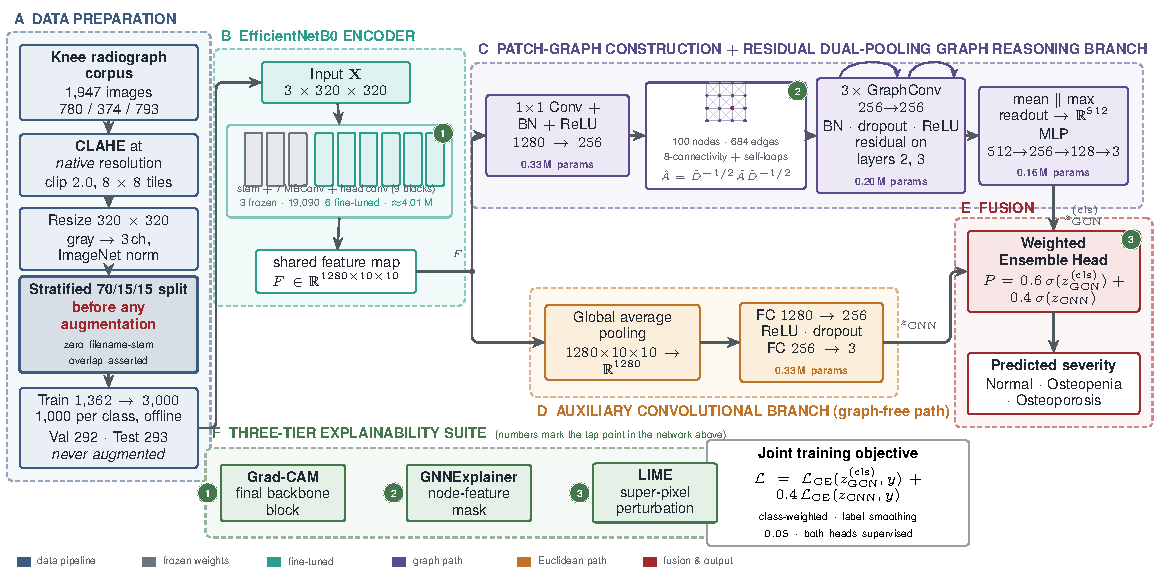
\includegraphics[width=\textwidth]{figs_vector/fig1_pipeline_overview.pdf}
    \caption{End-to-end EfficientNet-GCN pipeline. (A) The corpus is
    contrast-enhanced at native resolution and partitioned \emph{before} any
    augmentation, so no augmented variant of a validation or test radiograph can
    reach training. (B) An EfficientNetB0 trunk with its stem and first two
    MBConv stages frozen produces the shared feature map $F$. (C) $F$ is
    channel-reduced and reformulated as a 100-node, eight-connected patch graph
    that three residual graph-convolutional layers propagate over, read out by
    concatenated mean--max pooling. (D) In parallel, a graph-free branch pools
    $F$ directly. (E) The two class-probability vectors are fused
    $0.6/0.4$. (F) Three explanation methods tap the network at the numbered
    points. Parameter counts are given per component; the model totals 5.03\,M.}
    \label{fig:workflow_gcn}
\end{figure*}

\subsection{Dataset Description}
\label{sec:dataset}
The dataset consists of 1,947 knee radiographs distributed across three
diagnostic categories: Normal (780 images), Osteopenia (374 images), and
Osteoporosis (793 images) \cite{gobara2024multiclass}. The imbalance is
notable, with Osteopenia accounting for less than a fifth of the corpus, a
disparity that shaped the augmentation strategy of
Section~\ref{sec:augmentation}. Images were organized by class into separate
directories and read with a standard folder-labelled loader, so class
membership was inferred from directory structure rather than an external
annotation file.

The corpus is distributed as a public Kaggle dataset. Several properties
relevant to methodological interpretation are not documented by the source and
could not be recovered: the acquiring institution or institutions, patient
demographics, acquisition parameters, the qualifications of the annotators, and
whether the severity labels were established against DXA-derived $T$-scores or
by radiographic reading alone. Critically, the distribution provides no
patient-level identifiers, so it cannot be determined whether any patient
contributed more than one radiograph, for example a bilateral pair or a
follow-up study. The consequences of these unknowns for the evaluation protocol
are addressed directly in Sections~\ref{sec:split} and~\ref{sec:limitations}.

\subsection{Data Preprocessing}
\label{sec:preprocessing}
Every image was first converted to grayscale, and CLAHE
\cite{zuiderveld1994contrast} (clip limit $2.0$, tile grid $8 \times 8$) was
applied \emph{at the image's native resolution}, before any resizing. This
ordering is deliberate: enhancing contrast first and resizing second preserves
the fine trabecular striations that carry much of the diagnostic signal in
bone-density assessment, whereas resizing first and enhancing contrast
afterwards would let CLAHE amplify resampling artefacts rather than genuine bone
structure. No denoising filter is applied, since a low-pass step before resizing
would smooth away the same trabecular texture. The contrast-enhanced image is
then resized to $320 \times 320$ pixels using area interpolation when downscaling
or cubic interpolation when upscaling, and the single grayscale channel is
replicated across three channels to match the input expectations of an
ImageNet-pretrained backbone.

An input resolution of $320 \times 320$ was chosen rather than EfficientNetB0's
native $224 \times 224$ for two reasons: it preserves more of the
high-frequency trabecular detail that CLAHE is applied to enhance, and it
yields a $10 \times 10$ terminal feature map, giving a 100-node patch graph
whose spatial granularity is fine enough to distinguish sub-regions of the joint
while remaining small enough to keep the graph branch inexpensive. The effect of
this choice has not been ablated (Section~\ref{sec:limitations}).

The choice of enhancement parameters was informed by a preliminary
bone-intensity analysis across the three classes, computing the mean and
standard deviation of grayscale pixel intensity per class
(Fig.~\ref{fig:intensity}). Class-wise means were \PEND\ (Normal), \PEND\
(Osteopenia), and \PEND\ (Osteoporosis), with standard deviations \PEND, \PEND,
and \PEND\ respectively; a Kruskal--Wallis test across the three groups gave
\PEND. This analysis surfaced a measurable, if modest, intensity gradient
across the classes, which supported the use of a local, tile-based contrast
method rather than a single global histogram stretch. At load time, images are
normalized using standard ImageNet statistics (mean $0.485, 0.456, 0.406$;
standard deviation $0.229, 0.224, 0.225$).

\begin{figure}[!t]
    \centering
    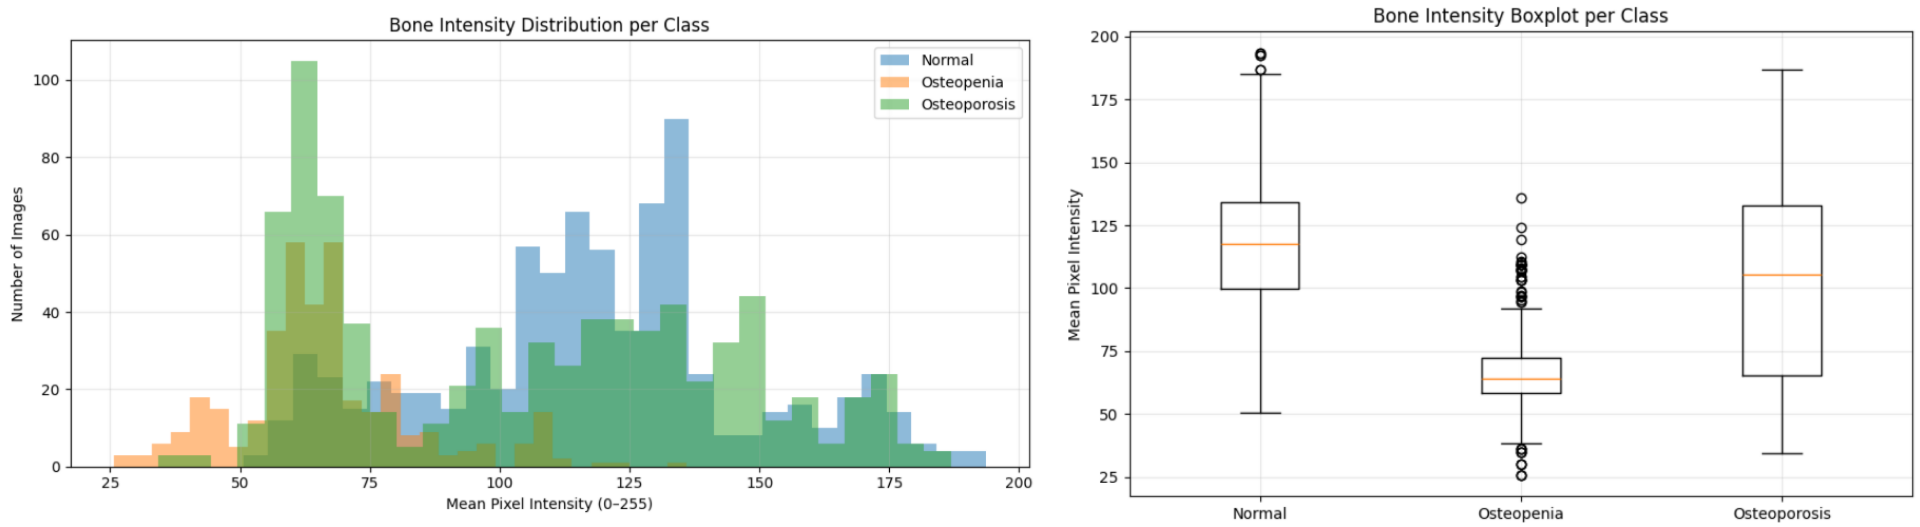
\includegraphics[width=.9\columnwidth]{bone_intensity_distribution.png}
    \caption{Bone intensity distribution per class.}
    \label{fig:intensity}
\end{figure}

\begin{figure}[!t]
    \centering
    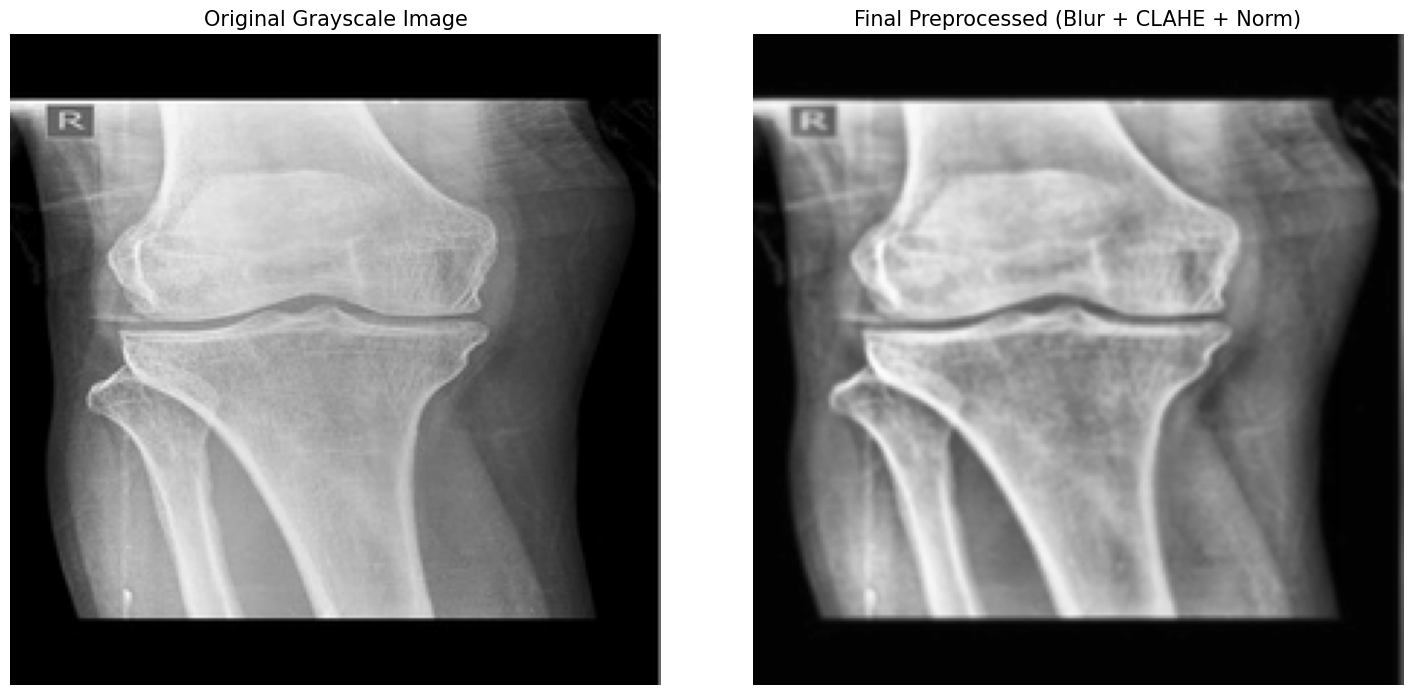
\includegraphics[width=.75\columnwidth]{preprocessed_comparison.png}
    \caption{Original versus preprocessed radiograph (CLAHE at native
    resolution, then resized).}
    \label{fig:preprocessed}
\end{figure}

\subsection{Dataset Split}
\label{sec:split}
Unlike a design that augments first and partitions second, the split here is
performed \emph{before} any augmentation, directly on the preprocessed
originals: each class is divided 70/15/15 into training, validation, and test
partitions (Table~\ref{tab:dataset_split}), yielding 1,362 training, 292
validation, and 293 test images. This ordering matters methodologically.
Augmenting before splitting can place near-duplicate variants of the same source
radiograph in both the training and test partitions, so that reported accuracy
partly reflects memorization of a specific radiograph rather than generalization
to an unseen one. Splitting first guarantees that every source radiograph
appears in exactly one partition; this was verified programmatically by
asserting zero filename-stem overlap between the train, validation, and test
directories after the split, and again after augmentation.

This check establishes that no \emph{image} appears in more than one partition.
It does not establish that no \emph{patient} does, because the source
distribution carries no patient identifiers (Section~\ref{sec:dataset}). If the
corpus contains bilateral pairs or repeat studies from the same individual, an
image-level partition can still leak patient identity across partitions, and the
reported test metrics would be correspondingly optimistic. This residual risk
cannot be excluded with the metadata available and is restated as a limitation
in Section~\ref{sec:limitations}.

Only the training partition is subsequently rebalanced by augmentation
(Section~\ref{sec:augmentation}); the validation and test partitions are left at
their natural, imbalanced class distribution and are evaluated using only the
deterministic preprocessing of Section~\ref{sec:preprocessing}, with every
metric reported as a macro average (Section~\ref{sec:metrics}) precisely because
the test set is not class-balanced.

\begin{table}[!t]
\centering
\caption{Dataset distribution: original 70/15/15 split, then training-only
augmentation}
\label{tab:dataset_split}
\begin{tabular}{@{}l c c c c@{}}
\toprule
\textbf{Class} & \textbf{Train (orig.)} & \textbf{Val} & \textbf{Test} &
\textbf{Train (aug.)} \\
\midrule
Normal        & 546  & 117 & 117 & 1000 \\
Osteopenia    & 261  & 56  & 57  & 1000 \\
Osteoporosis  & 555  & 119 & 119 & 1000 \\
\midrule
\textbf{Total} & \textbf{1362} & \textbf{292} & \textbf{293} & \textbf{3000} \\
\bottomrule
\end{tabular}
\end{table}

\subsection{Class-Balancing Augmentation}
\label{sec:augmentation}
Given the roughly two-to-one disparity between the smallest and largest classes
in the training partition, training directly on the raw distribution risked
biasing the classifier toward the majority classes. Rather than reweighting the
loss alone, the training partition itself was rebalanced through targeted,
offline augmentation, applied only after the split of Section~\ref{sec:split}
and only to the training images. Every original training image is retained
unchanged, and each class is then topped up with augmented variants, cycling
back through the originals as needed, until it reaches 1,000 images. An
Albumentations \cite{buslaev2020albumentations} pipeline supplies the augmented
variants, drawing from horizontal flip ($p=0.5$), a combined affine transform
with scaling in $[0.90,1.10]\times$, translation up to $6\%$ per axis, and
rotation within $\pm12^{\circ}$ ($p=0.8$), brightness/contrast jitter
($p=0.5$), and additive Gaussian noise ($p=0.3$). Each transform is applied
independently at its own probability rather than exactly one per image, so an
augmented sample may combine several perturbations. This step brings the
training partition to 1,000 images per class, 3,000 in total
(Table~\ref{tab:dataset_split}); the validation and test partitions are never
augmented.

A second, online augmentation stage is applied on top of this balanced training
set at every training step, implemented with torchvision transforms: random
resized cropping (scale $[0.85,1.0]$), random horizontal flip, random rotation
up to $10^{\circ}$, brightness/contrast jitter, and random erasing ($p=0.25$).
Random erasing is retained at a low probability as a mild occlusion-robustness
measure; because it can in principle occlude diagnostically relevant bone
regions, its net effect on this task has not been isolated and is listed among
the unablated design choices in Section~\ref{sec:limitations}. Hue and
saturation jitter are deliberately excluded, since the radiographs are grayscale
replicated across three channels and colour perturbations would desynchronize
the channels into hues that cannot occur in a real radiograph. Validation and
test images instead pass through a fixed, deterministic pipeline of resizing to
$320\times320$ followed by ImageNet normalization only, with no stochastic
transform of any kind.

\subsection{Framework Overview and Forward Pass}
\label{sec:overview}
EfficientNet-GCN is organized around three named components, described in turn
in Sections~\ref{sec:encoder}--\ref{sec:auxensemble}: a \textbf{Patch-Graph
Construction Module} that channel-reduces and turns the backbone's spatial
feature map into a relational patch graph, a \textbf{Residual Dual-Pooling Graph
Reasoning Branch} that propagates information across that graph and reads it
out, and an \textbf{Auxiliary Convolutional Branch} whose prediction is fused
with the graph branch's prediction by a \textbf{Weighted Ensemble Head}.
Fig.~\ref{fig:workflow_gcn} summarizes the resulting dataflow.

Let $\mathbf{X} \in \mathbb{R}^{3\times320\times320}$ denote a preprocessed input
image, $E_{\theta}(\cdot)$ the EfficientNetB0 encoder of
Section~\ref{sec:encoder}, $\mathrm{Proj}(\cdot)$ the channel-reduction step and
$\mathrm{PatchGraph}(\cdot)$ the graph-construction operator of
Section~\ref{sec:patchgraph}, $\mathrm{GCN}_3(\cdot)$ and
$\mathrm{DualPool}(\cdot)$ the three-layer graph branch and its readout from
Section~\ref{sec:gcnbranch}, and $\mathrm{MLP}_{\text{graph}}(\cdot)$ and
$\mathrm{MLP}_{\text{aux}}(\cdot)$ the two branches' classification heads. The
forward pass can then be written compactly as

\begingroup
\small
\begin{equation}
\label{eq:forward}
\begin{aligned}
F &= E_{\theta}(\mathbf{X}), \\
F' &= \mathrm{Proj}(F), \qquad \mathcal{G} = \mathrm{PatchGraph}(F'), \\
z_{\text{GCN}} &= \mathrm{DualPool}\big(\mathrm{GCN}_3(\mathcal{G})\big), \\
z_{\text{GCN}}^{(\text{cls})} &= \mathrm{MLP}_{\text{graph}}(z_{\text{GCN}}), \\
z_{\text{CNN}} &= \mathrm{MLP}_{\text{aux}}\big(\mathrm{GAP}(F)\big), \\
P_{\text{final}} &= 0.6\,\mathrm{softmax}\big(z_{\text{GCN}}^{(\text{cls})}\big)
+ 0.4\,\mathrm{softmax}\big(z_{\text{CNN}}\big),
\end{aligned}
\end{equation}
\endgroup

where $F \in \mathbb{R}^{1280\times10\times10}$ is the spatial feature map shared
by both branches, $F' \in \mathbb{R}^{256\times10\times10}$ is its
channel-reduced counterpart, $\mathcal{G}=(\mathcal{V},\mathcal{E})$ is the
100-node patch graph of Section~\ref{sec:patchgraph}, and
$P_{\text{final}} \in \mathbb{R}^{3}$ is the final class-probability vector
reported in Section~\ref{results}. All tensor shapes follow the
channels-first convention. Throughout, $\phi(\cdot)$ denotes the ReLU
nonlinearity and $\mathrm{softmax}(\cdot)$ the softmax function; the two are
kept notationally distinct because both appear as activation functions in
different parts of the model.

The two branches deliberately consume different tensors: the graph branch
reasons over the channel-reduced $F'$, while the auxiliary branch pools the
full, un-reduced $F$ directly. This shared-backbone, dual-branch design lets the
graph branch reason relationally over patch neighbourhoods while the auxiliary
branch retains a direct, graph-free path from features to logits; the two views
are combined at the output by Eq.~\eqref{eq:ensemble}.

\subsection{EfficientNetB0 Radiographic Encoder}
\label{sec:encoder}
The shared encoder $E_{\theta}(\cdot)$ is EfficientNetB0
\cite{tan2019efficientnet}, initialized from ImageNet weights. Its convolutional
trunk consists of a stem followed by seven MBConv stages and a final
$1\times1$ head convolution, nine top-level blocks in total. Rather than
freezing the entire network or fine-tuning it wholesale, only the last six of
these nine blocks, the final five MBConv stages together with the head
convolution, were made trainable, leaving the stem and the first two MBConv
stages frozen at their ImageNet-pretrained weights; this compromise lets the
network adapt its higher-level filters to radiographic texture while leaving the
most generic low-level filters undisturbed. For an input of $320 \times 320$,
the backbone produces the spatial feature map
$F \in \mathbb{R}^{1280\times10\times10}$ that feeds both downstream branches.

\subsection{Patch-Graph Construction Module}
\label{sec:patchgraph}
Before graph construction, a $1\times1$ convolution channel-reduces the shared
feature map from 1,280 to 256 channels:

\begingroup
\small
\begin{equation}
\label{eq:proj}
F' = \phi\big(\mathrm{BN}(\mathrm{Conv}_{1\times1}(F))\big)
\in \mathbb{R}^{256\times10\times10}.
\end{equation}
\endgroup

This projection exists to control the graph branch's parameter count: a
graph-convolutional layer consuming the raw 1,280-channel features would require
a $1280 \times 1280$ weight matrix, roughly 1.64M parameters in a single layer,
whereas the $1\times1$ convolution performs the reduction with 0.33M parameters
and leaves each subsequent graph layer at $256 \times 256$, or 65.5K parameters.
Rather than pooling $F'$ directly, as a conventional CNN classifier would, the
Patch-Graph Construction Module treats each of the one hundred spatial positions
of $F'$ as a node $x_i \in \mathbb{R}^{256}$ of a graph
$\mathcal{G}=(\mathcal{V},\mathcal{E})$ with $|\mathcal{V}|=100$
(Fig.~\ref{fig:architecture}, panel A). Nodes are connected to their spatial
neighbours under an eight-connectivity scheme, so each patch is linked to its
orthogonal and diagonal neighbours alike (Fig.~\ref{fig:architecture}, panel B),
producing 684 directed edges over the $10 \times 10$ grid. The resulting
adjacency $A$ is made self-connected and symmetrically normalized before being
consumed by the graph branch (Fig.~\ref{fig:architecture}, panel C):

\begingroup
\small
\begin{equation}
\label{eq:norm}
\tilde{A} = A + \mathbf{I}_{N}, \qquad
\tilde{D} = \mathrm{diag}\Big(\textstyle\sum_{j}\tilde{A}_{ij}\Big), \qquad
\hat{A} = \tilde{D}^{-\frac{1}{2}}\tilde{A}\tilde{D}^{-\frac{1}{2}},
\end{equation}
\endgroup

where $\mathbf{I}_{N}$ is the $N \times N$ identity matrix with $N=100$ and
$\tilde{D}$ is the degree matrix of the self-looped adjacency $\tilde{A}$. The
node set $\{x_i\}_{i=1}^{100}$ together with the normalized adjacency $\hat{A}$
constitutes the graph $\mathcal{G}$ consumed by the Residual Dual-Pooling Graph
Reasoning Branch of Section~\ref{sec:gcnbranch}.

A fixed adjacency was chosen over an attention-weighted alternative such as GAT
\cite{velickovic2018graph} or a learned $k$-nearest-neighbour construction
\cite{ye2025medgnn} because the neighbourhood structure of a regular grid is
known a priori and requires no parameters to represent. This design choice has a
significant analytical consequence, since the graph is then identical for every
input image; that consequence is examined in Section~\ref{sec:discussion}.

\begin{figure}[!t]
    \centering
    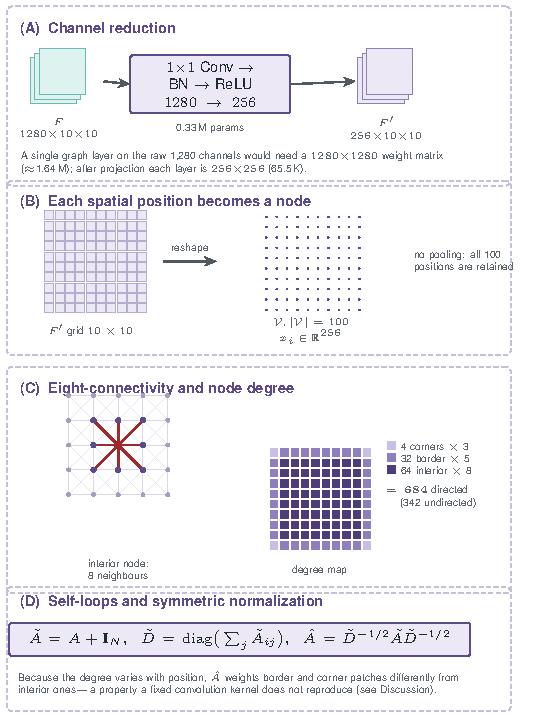
\includegraphics[width=\columnwidth]{figs_vector/fig2_patch_graph_module.pdf}
    \caption{Patch-Graph Construction Module. (A) A $1\times1$ convolution
    reduces the shared feature map from 1,280 to 256 channels
    (Eq.~\eqref{eq:proj}), which keeps each subsequent graph layer at
    $256\times256$ rather than $1280\times1280$. (B) Each of the 100 spatial
    positions becomes one node $x_i \in \mathbb{R}^{256}$; no pooling is
    applied. (C) Eight-connectivity links every patch to its orthogonal and
    diagonal neighbours. The degree map shows why the edge count is 684:
    4 corners of degree 3, 32 border patches of degree 5, and 64 interior
    patches of degree 8. (D) Self-loops are added and the adjacency is
    symmetrically normalized (Eq.~\eqref{eq:norm}); because degree varies with
    position, $\hat{A}$ weights border and interior patches differently.}
    \label{fig:architecture}
\end{figure}

\subsection{Residual Dual-Pooling Graph Reasoning Branch}
\label{sec:gcnbranch}
The patch graph $\mathcal{G}$ is processed by three stacked graph-convolutional
layers, all $256 \rightarrow 256$ since the channel reduction was already
performed by the Patch-Graph Construction Module (Eq.~\eqref{eq:proj}), each
following the first-order localized spectral propagation rule of Kipf and
Welling \cite{kipf2017semisupervised} (Fig.~\ref{fig:gcnbranch}):

\begingroup
\small
\begin{equation}
\label{eq:gcn}
H^{(l+1)} = \phi\left(\hat{A}\,H^{(l)}W^{(l)}\right),
\end{equation}
\endgroup

where $\hat{A}$ is the normalized self-looped adjacency of
Eq.~\eqref{eq:norm}, $H^{(l)}$ denotes the node features entering layer $l$
with $H^{(0)}$ the node set $\{x_i\}$, $W^{(l)}$ is the layer's learnable weight
matrix, and $\phi$ is the ReLU nonlinearity. Each layer is followed by batch
normalization, dropout, and $\phi$, with residual connections added around the
second and third layers to ease optimization as depth increases. Rather than
pooling the graph with a single readout, the branch concatenates a global
mean-pooling operation, capturing the overall density signal across the joint,
with a global max-pooling operation, capturing the single most abnormal patch:

\begingroup
\small
\begin{equation}
\label{eq:pooling}
z_{\text{GCN}} = \big[\,\mathrm{MeanPool}\big(H^{(3)}\big) \,;\,
\mathrm{MaxPool}\big(H^{(3)}\big)\,\big] \in \mathbb{R}^{512}.
\end{equation}
\endgroup

This 512-dimensional graph embedding then passes through a three-layer fully
connected head ($512 \rightarrow 256 \rightarrow 128 \rightarrow 3$) to produce
the graph branch's class logits $z_{\text{GCN}}^{(\text{cls})}$.

\begin{figure}[!t]
    \centering
    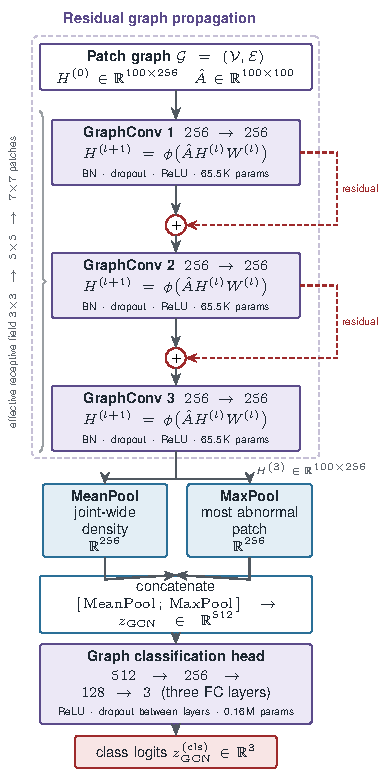
\includegraphics[width=\columnwidth]{figs_vector/fig3_gcn_branch.pdf}
    \caption{Residual Dual-Pooling Graph Reasoning Branch. Three
    graph-convolutional layers (Eq.~\eqref{eq:gcn}), each $256\to256$ with batch
    normalization, dropout, and ReLU, are stacked with residual connections
    around layers 2 and 3. Stacking three eight-connected propagations widens
    the effective receptive field from $3\times3$ to $7\times7$ patches. The
    resulting node features $H^{(3)}$ are read out by concatenated mean--max
    pooling (Eq.~\eqref{eq:pooling}), giving a 512-dimensional embedding that
    passes through the three-layer classification head to the class logits
    $z^{(\mathrm{cls})}_{\mathrm{GCN}}$.}
    \label{fig:gcnbranch}
\end{figure}

\subsection{Auxiliary Convolutional Branch and Weighted Ensemble Head}
\label{sec:auxensemble}
A second, considerably simpler branch operates in parallel on the same shared
feature map $F$, bypassing the graph entirely (Fig.~\ref{fig:auxensemble}):
global average pooling followed by two fully connected layers
($1280 \rightarrow 256 \rightarrow 3$) with a ReLU activation and dropout in
between, producing auxiliary logits $z_{\text{CNN}}$. This branch is trained
jointly with the graph branch, and the two predictions are combined at inference
by the Weighted Ensemble Head:

\begingroup
\small
\begin{equation}
\label{eq:ensemble}
P_{\text{final}} = w\cdot\mathrm{softmax}(z_{\text{GCN}}^{(\text{cls})})
+ (1-w)\cdot\mathrm{softmax}(z_{\text{CNN}}), \quad w = 0.6 .
\end{equation}
\endgroup

The larger weight is assigned to the graph branch on the grounds that it has
access to inter-patch relationships the auxiliary branch does not. The specific
value $w=0.6$ was fixed a priori rather than tuned, and was set to mirror the
auxiliary loss weight of Eq.~\eqref{eq:loss} for simplicity; no sensitivity
analysis over $w$ has yet been performed, and the sweep required to justify the
value empirically is reported as \PEND\ pending completion
(Section~\ref{sec:limitations}).

Because both heads share a single backbone and are optimized jointly through the
coupled objective of Eq.~\eqref{eq:loss}, this head is more precisely described
as a weighted probability fusion of two branches of one network than as an
ensemble of independently trained models; the term \emph{Weighted Ensemble Head}
is retained for consistency with the component naming used throughout.

\begin{figure}[!t]
    \centering
    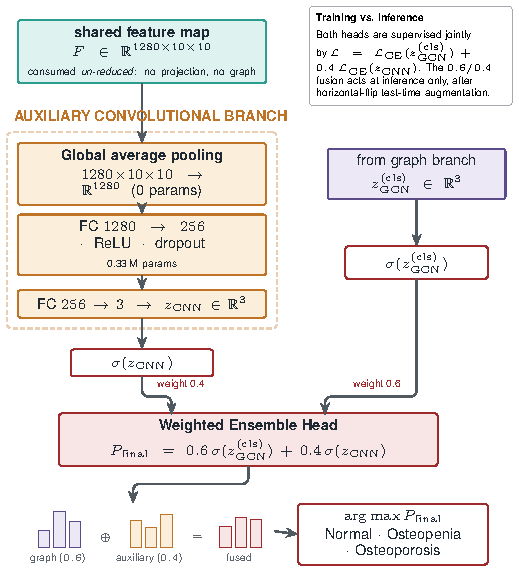
\includegraphics[width=\columnwidth]{figs_vector/fig4_auxiliary_ensemble.pdf}
    \caption{Auxiliary Convolutional Branch and Weighted Ensemble Head. The
    auxiliary branch consumes the shared feature map $F$ un-reduced, bypassing
    both the projection and the graph, and produces $z_{\text{CNN}}$ through
    global average pooling and two fully connected layers. Its softmax output is
    combined with the graph branch's $z_{\text{GCN}}^{(\text{cls})}$ by the
    $0.6/0.4$ weighted probability fusion of Eq.~\eqref{eq:ensemble},
    illustrated by the class-probability bars. Both heads are supervised jointly
    during training (Eq.~\eqref{eq:loss}); the fusion itself acts only at
    inference, after horizontal-flip test-time augmentation.}
    \label{fig:auxensemble}
\end{figure}

\subsection{Training Configuration}
\label{sec:training}
Training minimized a class-weighted cross-entropy loss with label smoothing,
combined with a secondary cross-entropy term on the auxiliary branch. Writing
$\tilde{y}_c = (1-\epsilon)\,\mathbb{1}[c = y] + \epsilon/C$ for the smoothed
target with $\epsilon = 0.05$ and $C = 3$, and $\omega_c$ for the
inverse-frequency class weight of class $c$, the per-branch objective and total
loss are

\begingroup
\small
\begin{equation}
\label{eq:loss}
\begin{aligned}
\mathcal{L}_{\text{CE}}(z, y) &= -\sum_{c=1}^{C} \omega_c\,\tilde{y}_c\,
\log \mathrm{softmax}(z)_c, \\
\mathcal{L} &= \mathcal{L}_{\text{CE}}(z_{\text{GCN}}^{(\text{cls})}, y)
+ \lambda_{\text{aux}}\,\mathcal{L}_{\text{CE}}(z_{\text{CNN}}, y),
\end{aligned}
\end{equation}
\endgroup

with $\lambda_{\text{aux}} = 0.4$. Because the training partition is already
balanced by the augmentation of Section~\ref{sec:augmentation}, the
inverse-frequency weights $\omega_c$ are uniform in practice; they are retained
in the implementation so that the same objective can be applied unchanged to the
unbalanced variant used in ablation (v).

Optimization used AdamW \cite{loshchilov2019decoupled} with two parameter groups
at differential learning rates: the unfrozen backbone layers were updated at
$1 \times 10^{-4}$, while the projection layer, graph branch, and auxiliary
branch were grouped together and updated more aggressively at
$1 \times 10^{-3}$, both with a weight decay of $1 \times 10^{-4}$. A bare
cosine schedule at the backbone learning rate destabilizes the pretrained
weights in the first steps, so the learning-rate multiplier instead follows a
linear warmup over the first three epochs followed by a single cosine decay to
zero over the remaining 42 epochs, with no restarts:

\begingroup
\small
\begin{equation}
\label{eq:schedule}
\eta_t = \eta_{\text{base}} \times
\begin{cases}
\dfrac{t+1}{T_{\text{warm}}}, & t < T_{\text{warm}} \\[6pt]
\dfrac{1}{2}\Big(1+\cos\Big(\pi\,\dfrac{t-T_{\text{warm}}}
{T_{\max}-T_{\text{warm}}}\Big)\Big), & t \geq T_{\text{warm}}
\end{cases}
\end{equation}
\endgroup

with $T_{\text{warm}}=3$ warmup epochs and $T_{\max}=45$ total epochs. Gradients
were clipped at a norm of $5.0$ to guard against instability introduced by the
graph convolutions. Training used mixed precision throughout except inside the
graph branch, whose sparse scatter operations are run in full precision for
numerical stability. Training was stopped early if validation macro F1-score,
rather than validation accuracy, failed to improve for ten consecutive epochs;
macro F1 is the model-selection criterion because the validation partition is
naturally imbalanced (Section~\ref{sec:split}), and accuracy alone can favour a
model that neglects the minority Osteopenia class. At inference, predictions
were averaged across the original image and its horizontal mirror, a lightweight
test-time augmentation intended to reduce sensitivity to left--right
orientation. Table~\ref{tab:hyperparameters} summarizes the configuration.

\begin{table}[!t]
\centering
\caption{Training and inference configuration}
\label{tab:hyperparameters}
\footnotesize
\begin{tabular}{@{}l l@{}}
\toprule
\multicolumn{2}{c}{\textbf{Input and backbone}} \\
\midrule
Input size & $320 \times 320$ \\
Backbone & EfficientNetB0 (last 6 of 9 blocks trainable) \\
Projection & $1\times1$ conv, $1280\rightarrow256$ \\
Graph structure & $10\times10$ grid, 8-connectivity \\
Graph edges & 684 directed (342 undirected) \\
GCN depth & 3 layers, 256 hidden units \\
\midrule
\multicolumn{2}{c}{\textbf{Optimization}} \\
\midrule
Optimizer & AdamW (differential learning rates) \\
Backbone LR / head LR & $1\times10^{-4}$ / $1\times10^{-3}$ \\
Weight decay & $1\times10^{-4}$ \\
Scheduler & Warmup (3 ep.) + cosine decay, 45 ep. \\
Loss & Class-weighted CE, label smoothing $0.05$ \\
Auxiliary loss weight $\lambda_{\text{aux}}$ & 0.4 \\
Batch size & 24 \\
Mixed precision & Enabled (except graph branch) \\
Gradient clip norm & 5.0 \\
Checkpoint selection & Best validation macro F1 \\
Early-stopping patience & 10 epochs \\
Random seed & \PEND \\
Independent runs & \PEND \\
\midrule
\multicolumn{2}{c}{\textbf{Inference}} \\
\midrule
Fusion weight $w$ & 0.6 (GCN), 0.4 (CNN) \\
Test-time augmentation & Horizontal-flip averaging \\
\bottomrule
\end{tabular}
\end{table}

\subsection{Experimental Setup}
\label{sec:expsetup}
All experiments were implemented in Python 3.12 using PyTorch 2.11 and PyTorch
Geometric (version \PEND) for the graph-convolutional layers, OpenCV for image
preprocessing, Albumentations \cite{buslaev2020albumentations} for augmentation,
and scikit-learn for evaluation metrics. Training was carried out in a Google
Colab GPU runtime on a single NVIDIA Tesla T4 with \PEND\ GB of system RAM.

\subsection{Evaluation Metrics and Statistical Analysis}
\label{sec:metrics}
Model performance was quantified on the test set using accuracy, macro-averaged
precision, recall, and F1-score, together with a per-class classification
report, a confusion matrix, and one-versus-rest ROC curves summarized by a
macro-averaged AUC. All quantities follow their standard definitions as
implemented in scikit-learn. Precision, recall, and F1 are reported as macro
averages, weighting each class equally regardless of support, because the test
partition is deliberately left at its natural, imbalanced distribution
(Section~\ref{sec:split}).

Because the severity grades are ordered rather than merely categorical, two
ordinal measures are additionally reported. The quadratic weighted kappa
compares the observed agreement matrix $O$ against the agreement matrix $E$
expected by chance, penalizing disagreements by the square of their grade
distance:

\begingroup
\small
\begin{equation}
\label{eq:qwk}
\kappa_{w} = 1 - \frac{\sum_{i,j} w_{ij}O_{ij}}{\sum_{i,j} w_{ij}E_{ij}},
\qquad w_{ij} = \frac{(i-j)^{2}}{(C-1)^{2}} .
\end{equation}
\endgroup

The mean absolute grade error, $\frac{1}{N}\sum_{n}|\hat{g}_n - g_n|$ over
grades encoded as $0,1,2$, is reported alongside it. Both quantities distinguish
a single-grade misclassification from the clinically far costlier
Normal--Osteoporosis confusion, which nominal accuracy treats identically.

\label{sec:statistics}
Interval estimates for accuracy and per-class recall are computed as Wilson
score intervals at the 95\% level, which is preferred to the normal
approximation at the sample sizes involved here, particularly for the 57-image
Osteopenia partition. Confidence intervals derived in this way from the reported
counts are given in Section~\ref{sec:testperf}. Repeated-run variability, by
contrast, cannot be estimated from a single training run: the results reported
below come from one run with a single fixed partition, so no standard deviation
across seeds or folds is available. The multi-seed and cross-validation protocol
required to supply that estimate, together with paired significance testing
against the baselines of Table~\ref{tab:baselines}, is reported as \PEND\
pending completion and is stated as a limitation in
Section~\ref{sec:limitations}.

\subsection{Explainable Artificial Intelligence Techniques}
\label{sec:xai}
Three explainability methods were applied to the trained model, each addressing
a different level of granularity.

Grad-CAM \cite{gradcam} was computed over the final block of the EfficientNetB0
backbone using the graph branch's logits as the target signal. This
construction differs from the standard application of Grad-CAM to a
convolutional classifier: gradients propagate from
$z_{\text{GCN}}^{(\text{cls})}$ back through the classification head, the three
graph-convolutional layers, and the $1\times1$ projection before reaching the
target activation map, so the resulting saliency reflects the graph branch's use
of the backbone features rather than a purely convolutional decision path.

GNNExplainer \cite{ying2019gnnexplainer} was applied to the trained graph head,
learning a soft mask over node features to identify which of the one hundred
patches most influenced a given prediction. Because the adjacency of
Section~\ref{sec:patchgraph} is fixed and identical for every input, the edge
mask that GNNExplainer also produces is defined over a topology that does not
vary across images and is therefore not informative for per-image comparison;
only the node-feature mask is reported here.

LIME \cite{lime} was used to generate super-pixel-level explanations by
perturbing the input image and observing the resulting change in the fused
output probabilities of Eq.~\eqref{eq:ensemble}, isolating both the regions that
supported a prediction and those that argued against it.

Feature-attribution methods such as SHAP \cite{lundberg2017unified} were
considered as a fourth complementary view but were not included, since Shapley
value estimation is substantially more expensive at the patch-graph resolution
used here; extending the suite to include SHAP is left for future work.

\section{Results}\label{results}
This section reports training behaviour, test-set performance, discriminative
power and error analysis, the ablation protocol, comparison with prior work, and
explainability outcomes.

\subsection{Training Behaviour}
Training ran for a maximum of 45 epochs but was stopped early at epoch 41 after
ten consecutive epochs without improvement in validation macro F1, the
model-selection criterion (Section~\ref{sec:training}). Training accuracy rose
from 63.77\% in epoch 1 to 93.30\% at epoch 41, while validation accuracy rose
from 69.18\% to a peak of 87.33\% at epoch 31, the checkpoint retained for final
evaluation, at which validation macro F1 reached 85.96\%. Training and
validation loss declined together over the same span, from 1.21 to 0.45 on the
training partition and from 0.98 to 0.66 on the validation partition, both
measured at the retained epoch-31 checkpoint. Comparing the two accuracies at
the final epoch gives a train--validation gap of 5.97 points, indicating mild
but controlled overfitting rather than either severe underfitting or
memorization. Fig.~\ref{fig:training-curves} depicts the training process.

\begin{figure}[!t]
    \centering
    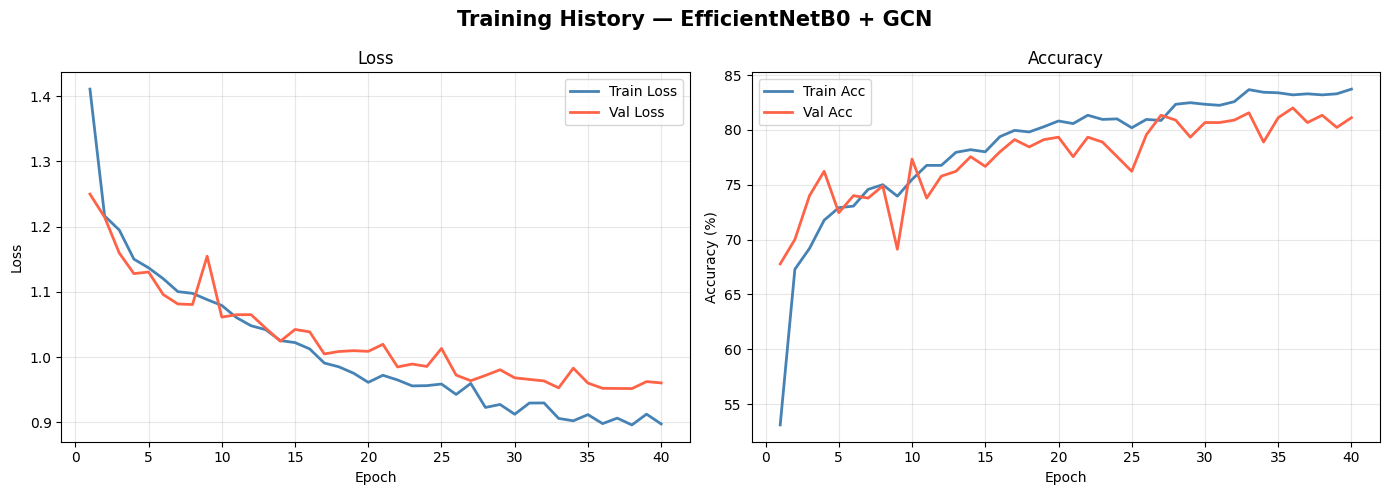
\includegraphics[width=.9\columnwidth]{gcn_training_curves.png}
    \caption{Training and validation loss and accuracy curves.}
    \label{fig:training-curves}
\end{figure}

\subsection{Test-Set Performance}
\label{sec:testperf}
On the 293-image held-out test set, held at its natural, imbalanced class
distribution (Section~\ref{sec:split}), the EfficientNet-GCN model achieved an
overall accuracy of 82.94\%, with macro-averaged precision, recall, and F1-score
of 0.8115, 0.8227, and 0.8161 respectively, as detailed in
Table~\ref{tab:overall_performance}.

The 95\% Wilson score interval for the overall accuracy is 78.21--86.81\%, a
span of roughly nine percentage points. This interval is wide because the test
partition contains only 293 images, and it should be borne in mind whenever the
headline figure is compared against values reported elsewhere. Per-class recall
intervals, given in Table~\ref{tab:per_class_performance}, are wider still, and
widest for Osteopenia, which is evaluated on 57 images.

\begin{table}[!t]
\centering
\caption{Overall test performance ($n = 293$)}
\label{tab:overall_performance}
\begin{tabular}{@{}l l@{}}
\toprule
\textbf{Metric} & \textbf{Value} \\
\midrule
Accuracy & 82.94\% (95\% CI 78.21--86.81) \\
Precision (macro) & 0.8115 \\
Recall (macro) & 0.8227 \\
F1-score (macro) & 0.8161 \\
AUC (macro, one-vs-rest) & 0.9429 \\
AUC (per class) & \PEND \\
Top-2 accuracy & \PEND \\
Quadratic weighted kappa & \PEND \\
Mean absolute grade error & \PEND \\
Expected calibration error & \PEND \\
\bottomrule
\end{tabular}
\end{table}

The per-class breakdown (Table~\ref{tab:per_class_performance}) shows the
strongest performance on the Normal class (precision 0.9107, recall 0.8718) and
the weakest on Osteopenia (precision 0.7031, recall 0.7895), which is
simultaneously the rarest class in the test set and, clinically, the
intermediate grade whose radiographic appearance sits closest to both of its
neighbours. Osteoporosis falls between the two (precision 0.8205, recall
0.8067). The pattern for Osteopenia, uniformly weaker precision and recall
rather than a strength in one and a weakness in the other, is consistent with
confusion concentrated at the two adjacent class boundaries rather than spread
evenly across all class pairs.

\begin{table}[!t]
\centering
\caption{Per-class test performance, with 95\% Wilson intervals on recall}
\label{tab:per_class_performance}
\footnotesize
\begin{tabular}{@{}l c c c c c@{}}
\toprule
\textbf{Class} & \textbf{Prec.} & \textbf{Rec.} & \textbf{95\% CI (rec.)} &
\textbf{F1} & \textbf{Support} \\
\midrule
Normal        & 0.9107 & 0.8718 & 0.799--0.921 & 0.8908 & 117 \\
Osteopenia    & 0.7031 & 0.7895 & 0.667--0.875 & 0.7438 & 57 \\
Osteoporosis  & 0.8205 & 0.8067 & 0.727--0.868 & 0.8136 & 119 \\
\midrule
\textbf{Macro avg} & \textbf{0.8115} & \textbf{0.8227} & --- &
\textbf{0.8161} & 293 \\
\bottomrule
\end{tabular}
\end{table}

\subsection{Discriminative Power and Error Analysis}
One-vs-rest ROC analysis yielded a macro-averaged AUC of 0.9429
(Fig.~\ref{fig:roc-curves}), indicating strong class separability despite the
more moderate hard-label accuracy. A gap of this size between ranking quality
and thresholded accuracy is consistent with a model whose probability estimates
order the three classes sensibly even where the arg-max decision is wrong. The
top-2 accuracy that would quantify this directly is reported as \PEND; until it
is available the interpretation should be treated as a hypothesis rather than an
established finding.

\begin{figure}[!t]
    \centering
    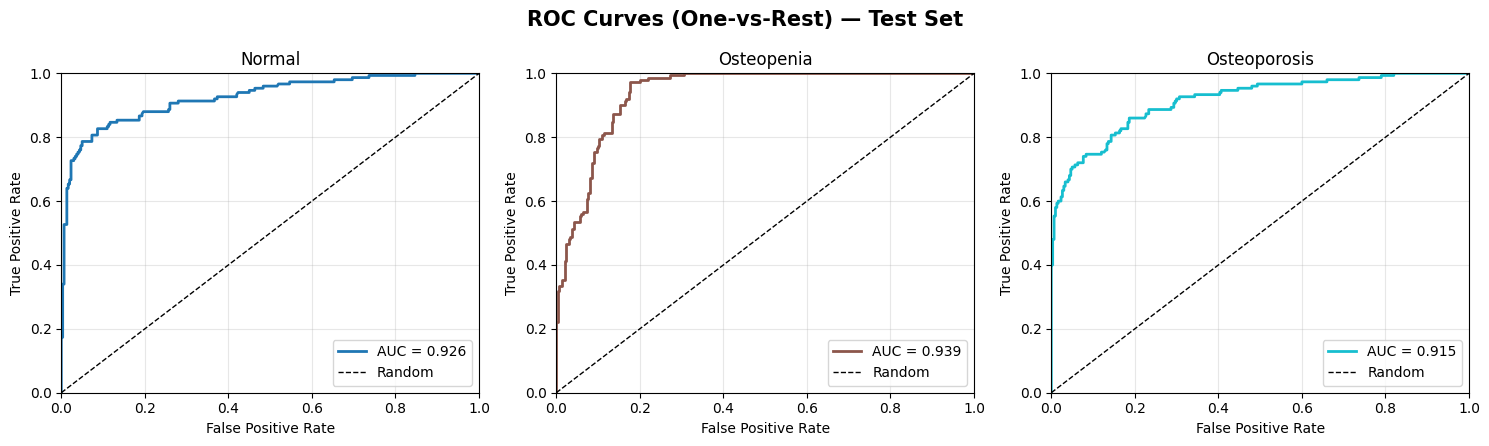
\includegraphics[width=.95\columnwidth]{gcn_roc_curves.png}
    \caption{One-vs-rest ROC curves per class, test set.}
    \label{fig:roc-curves}
\end{figure}

Fig.~\ref{fig:confusion-matrix} details the test-set confusion matrix. Of the
293 test predictions, 243 were correct and 50 were errors. Of those 50, 31 fall
on an adjacent-grade boundary (Normal--Osteopenia or Osteopenia--Osteoporosis),
while 19 fall on the Normal--Osteoporosis boundary, the costliest possible error
since it corresponds to a severe case read as entirely normal or the reverse.
Adjacent-grade confusions are therefore the more common failure mode, but the
19 extreme-boundary errors represent 38\% of all errors and 8\% of the 236
Normal and Osteoporosis test images combined. This is not a negligible residue,
and it is the single most important obstacle to clinical deployment of the model
in its current form; it motivates the ordinal-modelling direction set out in
Section~\ref{sec:futurework}.

\begin{figure}[!t]
    \centering
    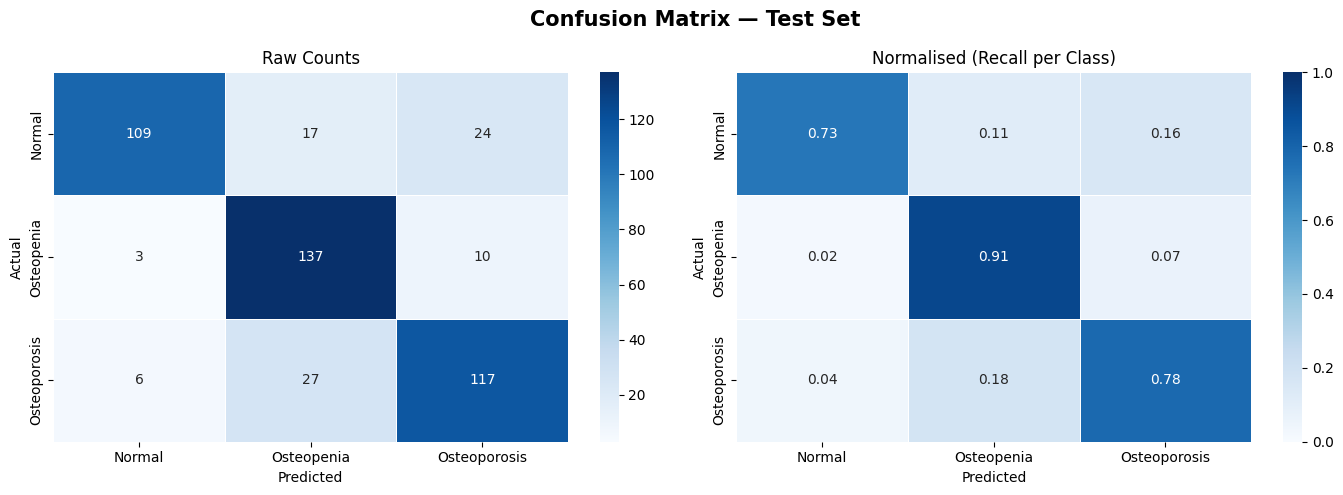
\includegraphics[width=.9\columnwidth]{gcn_confusion_matrix.png}
    \caption{Confusion matrix: raw counts and row-normalized recall, test set.}
    \label{fig:confusion-matrix}
\end{figure}

\subsection{Ablation Study}
\label{sec:ablation}
To isolate the contribution of each architectural and methodological component,
an ablation protocol was defined in which exactly one component of the pipeline
is removed or substituted at a time, while the data splits
(Table~\ref{tab:dataset_split}), backbone, and training budget
(Section~\ref{sec:training}) are held fixed for every variant. Seven variants are
defined: (i) \textit{w/o GCN branch}, in which the patch graph and its three
graph-convolutional layers are removed and the auxiliary branch alone produces
the prediction; (ii) \textit{w/o auxiliary branch}, in which the fusion of
Eq.~\eqref{eq:ensemble} is replaced by the graph branch's softmax output alone;
(iii) \textit{w/o dual pooling}, in which the concatenated mean--max readout is
replaced by mean pooling only; (iv) \textit{w/o CLAHE}, in which the
contrast-enhancement step of Section~\ref{sec:preprocessing} is skipped;
(v) \textit{w/o class-balancing augmentation}, in which the network is trained
on the original 546/261/555 training distribution; (vi) \textit{w/o test-time
augmentation}, in which inference uses a single forward pass; and
(vii) \textit{GCN branch replaced by a parameter-matched convolutional block},
in which the graph branch is substituted by a stack of $3\times3$ convolutions
with a comparable parameter budget operating on the same projected feature map
$F'$.

Variant (vii) is included specifically to control for model capacity. Because
the patch adjacency is fixed (Section~\ref{sec:patchgraph}), the propagation of
Eq.~\eqref{eq:gcn} aggregates over a $3\times3$ spatial neighbourhood at each
layer, and any accuracy gain attributed to relational reasoning must be shown to
exceed what an equally sized convolutional block achieves on the same features.
Without this control, variant (i) alone cannot distinguish a benefit of graph
structure from a benefit of added parameters.

Table~\ref{tab:ablation} lists these variants alongside the full model. At the
time of writing only the full-model row reflects a completed training run,
corresponding to the results reported in
Table~\ref{tab:overall_performance}; the remaining runs are pending. The
protocol is specified here in full so that each variant is reproducible from
Section~\ref{methodology}, and the incompleteness is stated plainly rather than
implied.

\begin{table}[!t]
\centering
\caption{Ablation protocol and results (test set, $n=293$)}
\label{tab:ablation}
\footnotesize
\begin{tabular}{@{}l c c c@{}}
\toprule
\textbf{Variant} & \textbf{Acc.} & \textbf{Macro F1} & \textbf{AUC} \\
\midrule
Full model (proposed) & 82.94\% & 0.8161 & 0.9429 \\
(i) w/o GCN branch & \PEND & \PEND & \PEND \\
(ii) w/o auxiliary branch & \PEND & \PEND & \PEND \\
(iii) w/o dual mean--max pooling & \PEND & \PEND & \PEND \\
(iv) w/o CLAHE preprocessing & \PEND & \PEND & \PEND \\
(v) w/o class-balancing augmentation & \PEND & \PEND & \PEND \\
(vi) w/o test-time augmentation & \PEND & \PEND & \PEND \\
(vii) GCN $\rightarrow$ param-matched conv & \PEND & \PEND & \PEND \\
\bottomrule
\end{tabular}
\end{table}

\subsection{Baselines Under an Identical Protocol}
\label{sec:baselines}
Cross-study accuracy comparisons confound architecture with dataset, class
count, and partitioning protocol. To separate these, Table~\ref{tab:baselines}
reports established backbones trained and evaluated under exactly the
preprocessing, partition, augmentation, and training budget described in
Section~\ref{methodology}. These runs are pending at the time of writing.

\begin{table}[!t]
\centering
\caption{Baselines trained under the identical protocol of
Section~\ref{methodology} (test set, $n=293$)}
\label{tab:baselines}
\scriptsize
\setlength{\tabcolsep}{4pt}
\begin{tabular}{@{}p{3.0cm} c c c c@{}}
\toprule
\textbf{Model} & \textbf{Acc.} & \textbf{Macro F1} & \textbf{AUC} &
\textbf{Params} \\
\midrule
EfficientNetB0 + GAP + FC & \PEND & \PEND & \PEND & \PEND \\
ResNet50 & \PEND & \PEND & \PEND & \PEND \\
DenseNet121 & \PEND & \PEND & \PEND & \PEND \\
VGG19 & \PEND & \PEND & \PEND & \PEND \\
Sarhan et al.~\cite{Sarhan2024} (reimpl.) & \PEND & \PEND & \PEND & \PEND \\
\midrule
\textbf{EfficientNet-GCN (proposed)} & \textbf{82.94\%} & \textbf{0.8161} &
\textbf{0.9429} & \textbf{5.03} \\
\bottomrule
\end{tabular}
\end{table}

\subsection{Computational Efficiency}
\label{sec:efficiency}
The proposed model contains 5,027,970 parameters (5.03M) in total, of which
5,008,880 (99.6\%) are trainable under the partial fine-tuning scheme of
Section~\ref{sec:encoder}. This figure was obtained directly from the trained
model rather than estimated, and breaks down as 4.01M in the EfficientNetB0
backbone, 0.33M in the projection layer, 0.36M in the graph branch, and 0.33M in
the auxiliary branch. Because the framework is motivated by deployment in
resource-constrained settings, parameter count alone is an insufficient measure
of cost; Table~\ref{tab:efficiency} lists the throughput measurements needed to
substantiate that motivation, which are pending.

\begin{table}[!t]
\centering
\caption{Computational cost of the proposed model}
\label{tab:efficiency}
\footnotesize
\begin{tabular}{@{}l l@{}}
\toprule
\textbf{Quantity} & \textbf{Value} \\
\midrule
Total parameters & 5,027,970 (5.03M) \\
Trainable parameters & 5,008,880 (99.6\%) \\
Multiply--accumulate operations & \PEND \\
GPU inference latency (T4, batch 1) & \PEND \\
CPU inference latency (batch 1) & \PEND \\
Peak inference memory & \PEND \\
\bottomrule
\end{tabular}
\end{table}

\subsection{Comparison with Prior Work}
\label{sec:comparison}
Table~\ref{tab:litreview} situates the proposed framework against published
deep-learning approaches to osteoporosis and BMD assessment across knee, hip,
spine, dental, and CT imaging. Raw accuracy figures in that table should be read
with caution rather than ranked directly: the compared studies differ in class
count, imaging modality, dataset size, label source, and partitioning protocol,
all of which affect the difficulty of the underlying decision problem. The
proposed model's 82.94\% accuracy carries a 95\% confidence interval of
78.21--86.81\% (Section~\ref{sec:testperf}), which overlaps several of the
figures below it in the table.

Three comparisons within the three-class knee-radiograph setting warrant direct
comment, since that is the setting most similar to the present one.

First, Sarhan et al.\ \cite{Sarhan2024} report 97.50\% on the same 1,947-image
corpus, 14.6 points above the present result and the highest figure reported for
this dataset. That study is also a three-class knee-radiograph formulation, so
the difference cannot be attributed to an easier decision problem. One
methodological difference is that the augmented corpus is partitioned after
augmentation rather than before, which permits variants of a single radiograph
to appear in both training and evaluation partitions; the present protocol
partitions first (Section~\ref{sec:split}). Whether this accounts for some,
all, or none of the 14.6-point margin cannot be determined without
reimplementing that pipeline under both orderings. That reimplementation is
listed as a baseline in Table~\ref{tab:baselines} and is pending; until it is
complete, no causal claim is made here, and the gap stands unexplained.

Second, Wani and Arora \cite{wani2023osteoporosis} report 91.10\% on a
three-class knee corpus, also above the present result, though on a
substantially smaller cohort of 381 images, where the corresponding confidence
interval would be wider still.

Third, the present result is comparable to Naguib et al.'s
\cite{Naguib2024} 83.74\% on a 611-image knee corpus, and exceeds Feng et al.'s
\cite{Feng2024} 74.00\% on a 139-image hip cohort.

The proposed framework therefore does not lead this literature on accuracy, and
is not claimed to. Its contribution is instead threefold and orthogonal to the
accuracy ranking: an explicit relational representation over patch-level
features rather than a purely Euclidean one; a partition-before-augment protocol
that removes a specific and widely present source of optimistic bias; and the
joint reporting of three complementary explanation views alongside a full
parameter budget, in a literature where no reviewed study reports a parameter
count at all. Whether any reviewed study reports more than a single explanation
method is recorded in the final column of Table~\ref{tab:litreview}.
Establishing that the relational component is
responsible for any part of the performance obtained requires the ablation of
Table~\ref{tab:ablation} and the baselines of Table~\ref{tab:baselines}, both
pending.

\subsection{Explainability Results}
Grad-CAM, computed on the final EfficientNetB0 block, localized activations over
cortical and medullary bone regions for the correctly classified Osteopenia and
Osteoporosis cases examined, rather than diffusing over background or soft
tissue (Fig.~\ref{fig:gradcam}). GNNExplainer, applied to the graph head,
identified a small, spatially contiguous cluster of patch-graph nodes as the
dominant contributors to each prediction examined
(Fig.~\ref{fig:gnnexplainer}). LIME's super-pixel explanations
(Fig.~\ref{fig:lime}) were broadly consistent with the Grad-CAM findings, with
positive regions concentrating over trabecular and cortical structures for both
Osteopenia and Osteoporosis predictions.

Two qualifications apply to these observations. First, they are qualitative
assessments of a selected set of correctly classified cases; no quantitative
faithfulness measure was computed, and no explanations of misclassified cases
were examined, so the evidence available cannot exclude the possibility that the
same methods would produce equally plausible-looking maps for incorrect
predictions. Deletion and insertion AUC scores for each of the three methods,
together with explanations of representative failure cases, are reported as
\PEND. Second, no clinician has reviewed the explanations, so their agreement
with expert judgement of which regions carry diagnostic signal is untested.
Accordingly, the results in this section are stated as consistency with
anatomically plausible regions, not as confirmation that the model reasons
clinically.

\begin{figure}[!t]
    \centering
    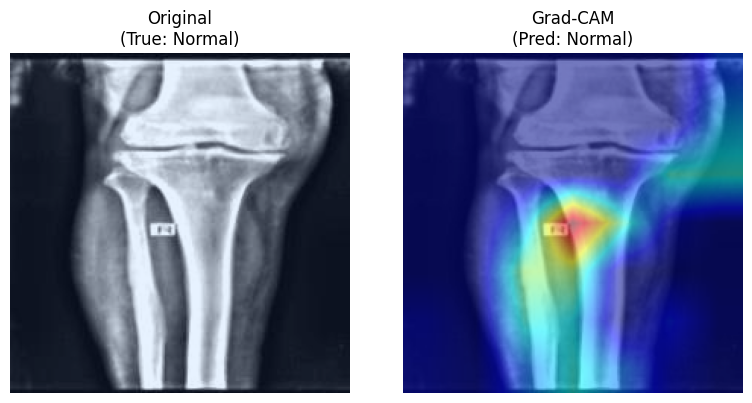
\includegraphics[width=.85\columnwidth]{gradcam_examples.png}
    \caption{Grad-CAM activation overlays on representative test samples.}
    \label{fig:gradcam}
\end{figure}

\begin{figure}[!t]
    \centering
    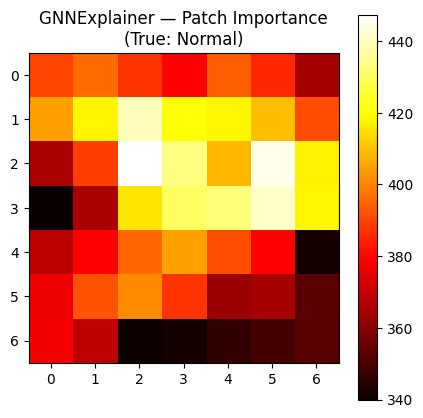
\includegraphics[width=.85\columnwidth]{gnn_explainer_overlay.png}
    \caption{GNNExplainer patch-importance heatmap and overlay on the original
    radiograph.}
    \label{fig:gnnexplainer}
\end{figure}

\begin{figure}[!t]
    \centering
    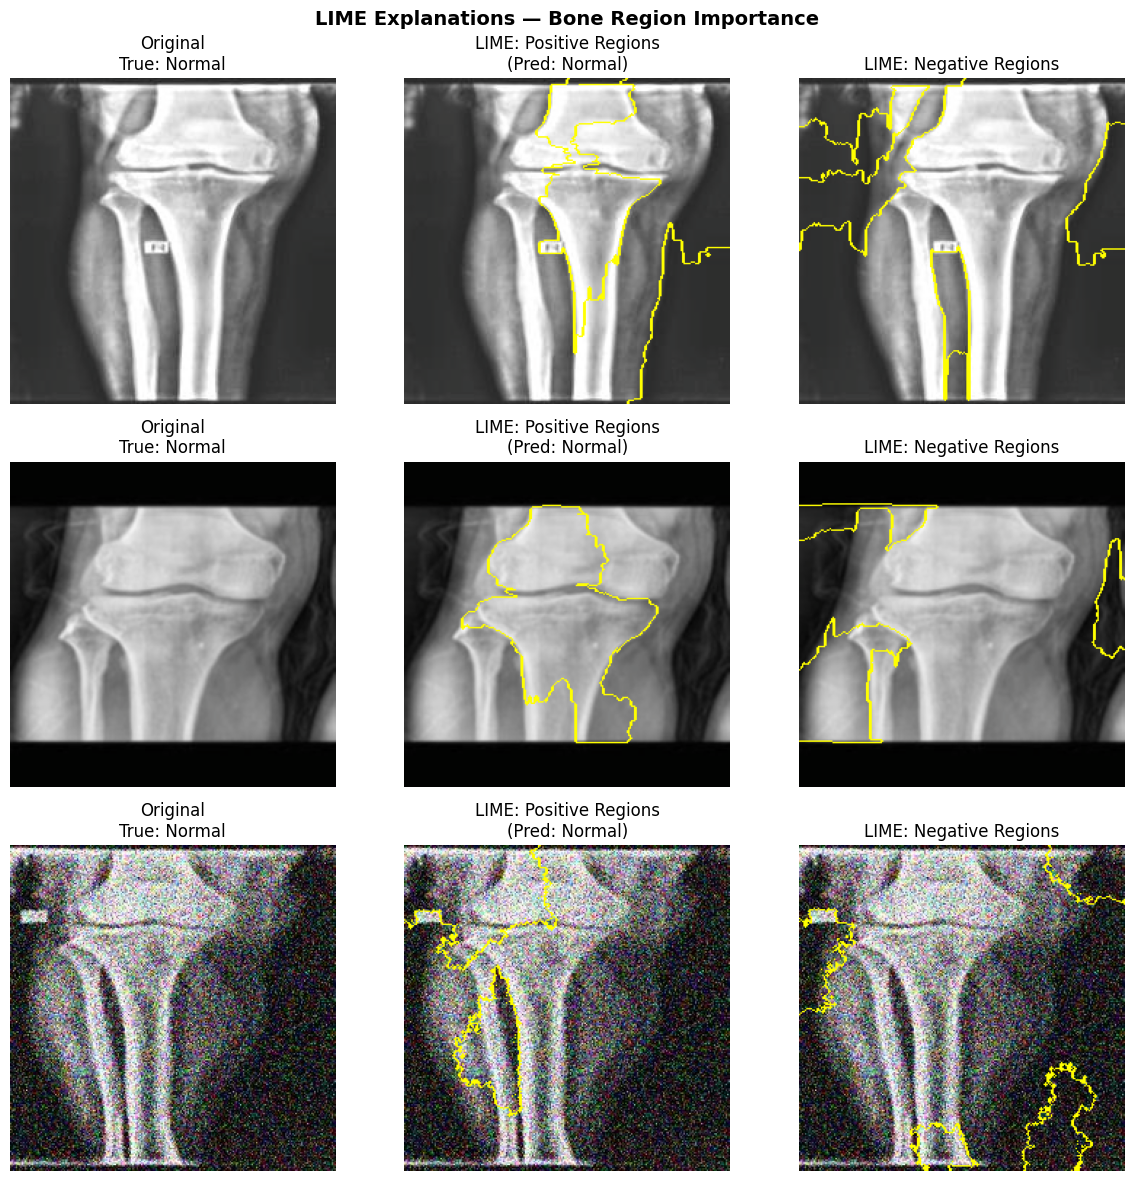
\includegraphics[width=.9\columnwidth]{lime_bone_explanations.png}
    \caption{LIME positive and negative super-pixel explanations across three
    test samples.}
    \label{fig:lime}
\end{figure}

\section{Discussion}
\label{sec:discussion}

\subsection{Where the Model Fails, and Why}
The error structure reported in Section~\ref{results} is coherent with the
clinical structure of the task. Osteopenia is both the rarest class in the test
partition and the intermediate grade, defined by a $T$-score band lying between
the other two, and it is the class on which the model is weakest in both
precision and recall. A classifier trained with a nominal cross-entropy
objective treats the three grades as unordered categories, so it receives no
signal that confusing Normal with Osteoporosis is worse than confusing either
with Osteopenia. The 19 extreme-boundary errors observed are the direct
consequence of that modelling choice. This suggests the task is better posed as
an ordinal regression problem than as a three-way nominal classification, a
direction taken up in Section~\ref{sec:futurework}.

\subsection{Does the Patch Graph Do Anything a Convolution Cannot?}
The most substantial theoretical objection to the present design concerns the
fixed adjacency. Because $A$ is an eight-connected lattice identical for every
input image, the propagation of Eq.~\eqref{eq:gcn} computes, at each node, a
degree-normalized sum over that node's $3\times3$ spatial neighbourhood followed
by a shared linear map. This is structurally close to a $3\times3$ convolution
whose kernel weights are fixed and tied across positions rather than learned,
and the objection follows that the graph branch may be reproducing an operation
the convolutional backbone already performs, with the apparent benefit coming
from the additional 0.36M parameters rather than from relational reasoning.

Three properties distinguish the two operations. The symmetric normalization
$\tilde{D}^{-1/2}\tilde{A}\tilde{D}^{-1/2}$ makes each node's aggregation
degree-dependent, so patches at the grid boundary and corners, which have five
and three neighbours respectively rather than eight, are weighted differently
from interior patches, whereas a convolution applies an identical kernel
everywhere and handles boundaries by padding. Stacking three such layers yields
an effective receptive field spanning a $7\times7$ patch region, which at this
feature-map scale covers a substantial fraction of the joint. And the
formulation generalizes directly to a learned or feature-dependent adjacency,
which a fixed convolution does not.

These are arguments for a difference in principle. They are not evidence of a
difference in effect on this task, and the present results do not supply that
evidence: variant (vii) of Table~\ref{tab:ablation} is precisely the experiment
that would settle it, and it is pending. Until it is run, the claim that
relational reasoning contributes to the reported performance should be regarded
as motivated but unverified. This is stated explicitly because it is the
manuscript's principal methodological vulnerability, and because the
alternative, a learned adjacency of the kind used by MedGNN
\cite{ye2025medgnn} or an attention-weighted formulation \cite{velickovic2018graph},
would make the relational component parametrically irreducible to a convolution
and is the natural next step (Section~\ref{sec:futurework}).

\subsection{Ranking Quality Versus Decision Quality}
The macro AUC of 0.9429 alongside 82.94\% accuracy indicates that the model's
class rankings are considerably better than its arg-max decisions. Two
non-exclusive explanations are available: the decision rule may be miscalibrated,
in which case threshold adjustment on the validation partition would recover
accuracy without retraining, or the fixed fusion weight $w=0.6$ of
Eq.~\eqref{eq:ensemble} may be suboptimal, since it was set a priori rather than
tuned. Both are cheap to test and neither has been tested here. The calibration
error and the fusion-weight sweep reported as \PEND\ would distinguish them.

\subsection{Clinical Positioning}
The framework is positioned as a triage aid rather than a diagnostic
replacement. In a screening pathway, its plausible role is to flag radiographs
warranting DXA referral, a binary decision, rather than to assign a definitive
severity grade. Reported three-class accuracy is not the metric that governs
performance in that role; sensitivity at a clinically acceptable specificity is.
The present evaluation does not report an operating-point analysis of this kind,
and adding one is a priority (Section~\ref{sec:futurework}). Any deployment
claim would additionally require the external validation the study lacks.

\section{Limitations}
\label{sec:limitations}
Seven limitations qualify the results reported above.

First, and most importantly for interpreting Table~\ref{tab:ablation}, seven of
the eight ablation variants remain unrun. The protocol is fully specified in
Section~\ref{sec:ablation}, but only the full model's row reflects a completed
training run, so no component of the architecture has yet been shown to
contribute to the reported performance.

Second, no baseline has been trained under the identical protocol
(Table~\ref{tab:baselines}). The comparison in Section~\ref{sec:comparison} is
therefore against figures obtained on different partitions and, in most cases,
different datasets, which does not isolate the effect of the proposed
architecture.

Third, the reported metrics come from a single training run on a single fixed
partition. No repeated-seed or cross-validation estimate of variance is
available, and no significance test against any alternative has been performed.
The Wilson intervals in Section~\ref{sec:testperf} capture sampling uncertainty
in the test partition but not variability across training runs or partitions.

Fourth, consistent with Gap 5 of Section~\ref{gaps}, the framework has been
evaluated on a single publicly distributed dataset \cite{gobara2024multiclass}
and has not been tested on independent, multi-centre clinical data, so its
generalization across scanners and acquisition protocols is unverified.

Fifth, the source dataset provides no patient-level identifiers
(Section~\ref{sec:dataset}). The partition was verified free of image-level
overlap, but if the corpus contains bilateral pairs or repeat studies from the
same individual, patient-level leakage cannot be excluded and the reported
metrics would be optimistic. This limitation applies to any study using this
corpus, including those the present work compares against.

Sixth, because the validation and test partitions are deliberately left at their
natural distribution, the Osteopenia class is evaluated on only 57 images, and
its recall interval spans 0.667--0.875 (Table~\ref{tab:per_class_performance}).
Conclusions about this class are correspondingly weak.

Seventh, radiographic severity labels were taken as provided by the source
dataset rather than confirmed against DXA-derived $T$-scores, so label noise at
the class boundaries the model confuses most often cannot be ruled out. Several
design choices, including the $320\times320$ input resolution, the random-erasing
augmentation, and the fusion weight $w = 0.6$, were also fixed a priori rather
than selected empirically.

\section{Future Work}
\label{sec:futurework}
Completing the ablation of Table~\ref{tab:ablation}, including the
parameter-matched convolutional control, and the identically trained baselines
of Table~\ref{tab:baselines} is the most immediate priority, since together they
determine whether the architectural claims of this paper hold. Repeating the
protocol across multiple seeds or cross-validation folds, with paired
significance testing, would supply the variance estimates the present results
lack.

Beyond this, five directions follow. Reformulating the task as ordinal
regression, through a CORAL-style cumulative-link head or a distance-weighted
loss, directly targets the extreme-boundary errors identified in
Section~\ref{sec:discussion} and matches the ordered structure of the severity
scale. Replacing the fixed eight-connectivity adjacency with a learned
edge-weighting scheme, following the attention-based formulation
\cite{velickovic2018graph} or the $k$-nearest-neighbour construction of MedGNN
\cite{ye2025medgnn}, would make the relational component parametrically distinct
from a convolution. Adding quantitative explanation-faithfulness measures and
radiologist review would convert the qualitative explainability findings into
evidence. Reporting a binary DXA-referral operating point, with sensitivity at a
fixed specificity, would evaluate the model in the clinical role actually
proposed for it. Finally, external multi-centre validation and the collection of
additional Osteopenia cases would address the two gaps this study inherits from
the wider literature.

\section{Conclusion} \label{conclusion}
This paper presented EfficientNet-GCN, a hybrid convolutional--graph framework
for osteoporosis severity classification from knee radiographs, built around a
Patch-Graph Construction Module, a Residual Dual-Pooling Graph Reasoning Branch,
and an Auxiliary Convolutional Branch fused through a Weighted Ensemble Head. An
ImageNet-pretrained EfficientNetB0 encoder extracts spatial features; the
Patch-Graph Construction Module channel-reduces and reformulates them into a
100-node, eight-connected graph; and the graph branch propagates relational
context across that graph, treating anatomically adjacent regions of the knee
joint as connected nodes rather than isolated units.

The corpus is partitioned before any augmentation is applied and only the
training partition is rebalanced, so the validation and test partitions retain
their natural class distribution and no augmented variant of a test radiograph
can appear in training. Under this protocol the model reaches 82.94\% accuracy
(95\% CI 78.21--86.81\%) and a macro one-vs-rest AUC of 0.9429 on the held-out
test set, with 5.03M parameters. Grad-CAM, GNNExplainer, and LIME localize
predictions to cortical and trabecular bone regions in the cases examined.

The framework does not exceed the best previously reported accuracy on this
corpus, and the present evidence does not yet establish that its relational
component is responsible for the performance obtained: the ablation of
Table~\ref{tab:ablation}, the parameter-matched convolutional control, and the
identically trained baselines of Table~\ref{tab:baselines} are all pending, and
Section~\ref{sec:discussion} sets out why the last of these is decisive. What
the study does contribute is a leakage-controlled evaluation protocol, an
explicit relational representation over patch-level features, and the joint
reporting of three complementary explanation views alongside a full parameter
budget, in a literature where at most one explanation method and no parameter
count are typically reported. Sections~\ref{sec:limitations}
and~\ref{sec:futurework} state the remaining gaps and the steps planned to close
them.

\section*{Data and Code Availability}
The knee radiograph dataset used in this study, the Multi-Class Knee
Osteoporosis X-Ray Dataset, is publicly available on Kaggle
\cite{gobara2024multiclass} at
\url{https://www.kaggle.com/datasets/mohamedgobara/multi-class-knee-osteoporosis-x-ray-dataset}.
% FIXME (C2): replace the sentence below with the repository URL once the code
% is released, or state explicitly that it is available on request.
Source code, the partition manifest, and the random seeds required to reproduce
the reported results are available at \PEND.

\section*{Ethical Statement}
This study used a publicly available, de-identified, third-party imaging dataset
\cite{gobara2024multiclass} and involved no prospective recruitment, no
intervention, and no access to identifiable patient information. Institutional
review board approval and informed consent were therefore not required. The
authors did not attempt to re-identify any individual represented in the data.

\section*{Conflict of Interest}
The authors declare no conflict of interest.

\section*{Author Contributions}
% FIXME: adjust to reflect the actual division of work before submission.
T. S. Sintheia: conceptualization, methodology, software, investigation,
writing---original draft. M. R. Muin: software, validation, data curation,
visualization. P. D. Gupta: investigation, formal analysis, visualization.
M. I. Mobin: supervision, methodology, writing---review and editing. All authors
read and approved the final manuscript.

\section*{Funding}
This research received no specific grant from any funding agency in the public,
commercial, or not-for-profit sectors.

\bibliographystyle{IEEEtran}
\bibliography{ref}

\end{document}
